\setcounter{section}{0}%更改chapter的计数器值
%\numberwithin{equation}{chapter}%公式计数器从属于节计数器
\numberwithin{equation}{section}%公式计数器从属于节计数器
\numberwithin{figure}{section}%图计数器从属于节计数器
\setcounter{chapter}{1}

%\chapter{\texorpdfstring{共形场论}{2 Conformal field theory}}
\chapter{共形场论}
本章手稿不全,2.1节和2.2节缺失一部分.

%\section{\texorpdfstring{2维无质量标量}{2.1 Massless scalars in two dimensions}}
\section{2维无质量标量}
因本节手稿不全(仅有公式2.1.18-2.1.24,前一半缺失),暂用英文原文代替.\\
We will start with the example of D free scalar fields in two dimensions,$X^{\mu}\left(\sigma^{1}, \sigma^{2}\right)$.
We will refer to these two dimensions as the world-sheet,
anticipating the application to string theory. The action is
\begin{equation}
S=\frac{1}{4 \pi \alpha^{\prime}} \int d^{2} \sigma\left(\partial_{1} X^{\mu} \partial_{1} X_{\mu}+\partial_{2} X^{\mu} \partial_{2} X_{\mu}\right)
\end{equation}
This is the Polyakov action (1.2.13), except that the world-sheet metric $\gamma_{a b}$ has been replaced with a flat Euclidean metric $\delta_{a b}$, signature $(+,+) .$ The overall sign change of the action is a result of the Euclidean convention (A.1.31). As we will see, most string calculations are carried out on a Euclidean world-sheet. At least for flat metrics, the relation between Euclidean and Minkowski amplitudes is given by a standard analytic continuation, explained in the appendix. In fact, the results of the present chapter apply equally to a Minkowski world-sheet, and in the first seven sections all equations make sense if $\sigma^{2}$ is replaced with $i \sigma^{0} .$ For the index $\mu$ we still take the flat Minkowski metric.\\

It is straightforward to quantize the action (2.1.1) canonically, finding the spectrum, vacuum expectation values, and so on. We have done essentially this in chapter 1 , after having gone to light-cone gauge. Here we will take a somewhat different route, developing first various local properties such
as equations of motion, operator products, Ward identities, and conformal
invariance, before working our way around to the spectrum. It will be
efficient for us to use the path integral formalism. This is reviewed in the
appendix. We will be using the path integral representation primarily to
derive operator equations (to be defined below); these can also be derived
in a Hilbert space formalism.
It is very useful to adopt complex coordinates
\begin{equation}
z=\sigma^{1}+i \sigma^{2}, \quad \bar{z}=\sigma^{1}-i \sigma^{2}
\end{equation}
We will use a bar for the complex conjugates of z and other simple
variables, and a star for the complex conjugates of longer expressions.
Define also
\begin{equation}
\partial_{z}=\frac{1}{2}\left(\partial_{1}-i \partial_{2}\right), \quad \partial_{\bar{z}}=\frac{1}{2}\left(\partial_{1}+i \partial_{2}\right)
\end{equation}
These derivatives have the properties
\begin{equation}
\partial_{z} z=1, \quad \partial_{z} \bar{z}=0, \quad \partial_{\bar{z}} z=0, \quad \partial_{\bar{z}} \bar{z}=1
\end{equation}
It is conventional to abbreviate $\partial_{z}$ to $\partial$ and $\partial_{\bar{z}}$ to $\bar{\partial}$ when this is not ambiguous. For a general vector $v^{a}$, define in the same way

\begin{equation}
v^{z}=v^{1}+i v^{2}, \quad v^{\bar{z}}=v^{1}-i v^{2}, \quad v_{z}=\frac{1}{2}\left(v^{1}-i v^{2}\right), \quad v_{\bar{z}}=\frac{1}{2}\left(v^{1}+i v^{2}\right)
\end{equation}

For the indices 1, 2 the metric is the identity and we do not distinguish
between upper and lower, while the complex indices are raised and lowered
with
\begin{equation}
g_{z \bar{z}}=g_{\bar{z} z}=\frac{1}{2}, \quad g_{z z}=g_{\bar{z} \bar{z}}=0, \quad g^{z \bar{z}}=g^{\bar{z} z}=2, \quad g^{z z}=g^{\bar{z} \bar{z}}=0
\end{equation}
Note also that
\begin{equation}
d^{2} z=2 d \sigma^{1} d \sigma^{2}
\end{equation}
with the factor of 2 from the Jacobian, ${ }^{1}$ and that $d^{2} z|\operatorname{det} g|^{1 / 2}=d \sigma^{1} d \sigma^{2}$. We define
\begin{equation}
\int d^{2} z \delta^{2}(z, \bar{z})=1
\end{equation}
so that $\delta^{2}(z, \bar{z})=\frac{1}{2} \delta\left(\sigma^{1}\right) \delta\left(\sigma^{2}\right) .$ Another useful result is the divergence
theorem in complex coordinates,
\begin{equation}
\int_{R} d^{2} z\left(\partial_{z} v^{z}+\partial_{\bar{z}} v^{\bar{z}}\right)=i \oint_{\partial R}\left(v^{z} d \bar{z}-v^{\bar{z}} d z\right)
\end{equation}
where the contour integral circles the region R counterclockwise.
In this notation the action is
\begin{equation}
S=\frac{1}{2 \pi \alpha^{\prime}} \int d^{2} z \partial X^{\mu} \bar{\partial} X_{\mu}
\end{equation}
and the classical equation of motion is
\begin{equation}
\partial \bar{\partial} X^{\mu}(z, \bar{z})=0
\end{equation}
The notation $X^{\mu}(z, \bar{z})$ may seem redundant, since the value of $z$ determines the value of $\bar{z}$, but it is useful to reserve the notation $f(z)$ for fields whose equation of motion makes them analytic (equivalently holomorphic) functions of $z$. Writing the equation of motion as
\begin{equation}
\partial\left(\bar{\partial} X^{\mu}\right)=\bar{\partial}\left(\partial X^{\mu}\right)=0
\end{equation}
it follows that $\partial X^{\mu}$ is holomorphic and that $\bar{\partial} X^{\mu}$ is antiholomorphic (holomorphic in $\bar{z}$ ), hence the notations $\partial X^{\mu}(z)$ and $\bar{\partial} X^{\mu}(\bar{z})$.

Under the Minkowski continuation $\sigma^{2}=i \sigma^{0}$, a holomorphic field becomes a function only of $\sigma^{0}-\sigma^{1}$ and an antiholomorphic field a function only of $\sigma^{0}+\sigma^{1}$. We thus use as synonyms
\begin{subequations}
\begin{equation}
\text { holomorphic }=\text { left-moving }
\end{equation}
\begin{equation}
\text { antiholomorphic }=\text { right-moving }
\end{equation}
\end{subequations}
This terminology is chosen to have maximal agreement with the literature, though for it to hold literally we would need to draw $\sigma^{1}$ increasing from right to left. We will tend to use the Euclidean terms early on and shift to the Minkowski terms as we discuss more of the spacetime physics. Expectation values are defined by the path integral,
\begin{equation}
\langle\mathscr{F}[X]\rangle=\int[d X] \exp (-S) \mathscr{F}[X]
\end{equation}
where $\mathscr{F}[X]$ is any functional of $X$, such as a product of local operators. The path integral over $X^{0}$ is a wrong-sign Gaussian, so it should be understood to be defined by the analytic continuation $X^{0} \rightarrow-i X^{D}$. The reader should not be distracted by this; we will discuss it further in the next chapter. We do not normalize $\langle\mathscr{F}[X]\rangle$ by dividing by $\langle 1\rangle .$

The path integral of a total derivative is zero. This is true for ordinary bosonic path integrals, which can be regarded as the limit of an infinite number of ordinary integrals, as well as for more formal path integrals as
with Grassmann variables. Then
\begin{equation}
\begin{aligned}
0 &=\int[d X] \frac{\delta}{\delta X_{\mu}(z, \bar{z})} \exp (-S) \\
&=-\int[d X] \exp (-S) \frac{\delta S}{\delta X_{\mu}(z, \bar{z})} \\
&=-\left\langle\frac{\delta S}{\delta X_{\mu}(z, \bar{z})}\right\rangle \\
&=\frac{1}{\pi \alpha^{\prime}}\left\langle\partial \bar{\partial} X^{\mu}(z, \bar{z})\right\rangle
\end{aligned}
\end{equation}
The same calculation goes through if we have arbitrary additional insertions ‘. . .’ in the path integral, as long as none of these additional insertions
is at z. Thus
\begin{equation}
\left\langle\partial \bar{\partial} X^{\mu}(z, \bar{z}) \ldots\right\rangle=0
\end{equation}
We can regard the additional insertions as preparing arbitrary initial and
final states (or we could do the same thing with boundary conditions).
The path integral statement (2.1.16) is thus the same as the statement in
the Hilbert space formalism that
\begin{equation}
\partial \bar{\partial} \hat{X}^{\mu}(z, \bar{z})=0
\end{equation}
holds for all matrix elements of the operator $\hat{X}^{\mu}(z, \bar{z}) .$ Thus we refer to relations that hold in the sense (2.1.16) as operator equations. The statement (2.1.17) is Ehrenfest's theorem that the classical equations of motion translate into operator equations.

----------------------------------------------------------------------------------------------------------

路径积分(2.1.16)中的记号 '...'暗含了插入是远离z的. 但考察插入恰好在z的情况也是有趣的
\begin{equation}
\begin{aligned}
0 &=\int[d X] \frac{\delta}{\delta X_{\mu}(z, \bar{z})}\left[\exp (-S) X^{v}\left(z^{\prime}, \bar{z}^{\prime}\right)\right] \\
&=\int[d X] \exp (-S)\left[\eta^{\mu v} \delta^{2}\left(z-z^{\prime}, \bar{z}-\bar{z}^{\prime}\right)+\frac{1}{\pi \alpha^{\prime}} \partial_{z} \partial_{\bar{z}} X^{\mu}(z, \bar{z}) X^{v}\left(z^{\prime}, \bar{z}^{\prime}\right)\right]\\
&=\eta^{\mu v}\left\langle\delta^{2}\left(z-z^{\prime}, \bar{z}-\bar{z}^{\prime}\right)\right\rangle+\frac{1}{\pi \alpha^{\prime}} \partial_{z} \partial_{\bar{z}}\left\langle X^{\mu}(z, \bar{z}) X^{v}\left(z^{\prime}, \bar{z}^{\prime}\right)\right\rangle
\end{aligned}
\end{equation}
即,运动方程在巧合点之外成立. 再一次在路径积分中插入"..."
\begin{equation}
\frac{1}{\pi \alpha^{\prime}} \partial_{z} \partial_{\bar{z}}\left\langle X^{\mu}(z, \bar{z}) X^{v}\left(z^{\prime}, \bar{z}^{\prime}\right) \ldots\right\rangle=-\eta^{\mu \nu}\left\langle\delta^{2}\left(z-z^{\prime}, \bar{z}-\bar{z}^{\prime}\right) \ldots\right\rangle
\end{equation}
因而
\begin{equation}
\frac{1}{\pi \alpha^{\prime}} \partial_{z} \partial_{\bar{z}} X^{\mu}(z, \bar{z}) X^{v}\left(z^{\prime}, \bar{z}^{\prime}\right)=-\eta^{\mu v} \delta^{2}\left(z-z^{\prime}, \bar{z}-\bar{z}^{\prime}\right)
\end{equation}
其作为一个算符方程成立.\\
在Hilbert空间体系下,路径积分中的乘积作为编时乘积出现,而$\delta$函数来自作用在编时乘积的导数. 这一联系在附录中进一步发展. 在自由场论中,引入正规序列的算符是有用的. 正规序列算符记为$: \mathscr{A}:$,定义如下:
\begin{subequations}
\begin{equation}
: X^{\mu}(z, \bar{z}):=X^{\mu}(z, \bar{z})
\end{equation}
\begin{equation}
: X^{\mu}\left(z_{1}, \bar{z}_{1}\right) X^{v}\left(z_{2}, \bar{z}_{2}\right):=X^{\mu}\left(z_{1}, \bar{z}_{1}\right) X^{v}\left(z_{2}, \bar{z}_{2}\right)+\frac{\alpha^{\prime}}{2} \eta^{\mu v} \ln \left|z_{12}\right|^{2}
\end{equation}
\end{subequations}
其中
\begin{equation}
z_{i j}=z_{i}-z_{j}
\end{equation}
读者也许熟悉以升降算符定义的正规序列. 这两个定义稍后将联系起来. \\
该定义的关键点是性质:
\begin{equation}
\partial_{1} \bar{\partial}_{1}: X^{\mu}\left(z_{1}, \bar{z}_{1}\right) X^{v}\left(z_{2}, \bar{z}_{2}\right):=0
\end{equation}
上式源于算符方程(2.1.20)以及如下微分方程
\begin{equation}
\partial \bar{\partial} \ln |z|^{2}=2 \pi \delta^{2}(z, \bar{z})
\end{equation}
由于 $\ln |z|^{2}=\ln z+\ln \bar{z}$,上式对于$z \neq 0$ 是显然的. 通过(2.1.9) 对两边积分很容易检验$\delta$ 函数的归一化.

\section{算符乘积展开}%{2.2 The operator product expansion}
因本节手稿不全(仅有公式2.2.1-2.2.4,后一半缺失),暂用英文原文代替.\\
弦微扰论是基本主题是定域算符之积的路径积分期望值
\begin{equation}
\left\langle\mathscr{A}_{i_{1}}\left(z_{1}, \bar{z}_{1}\right) \mathscr{A}_{i_{2}}\left(z_{2}, \bar{z}_{2}\right) \ldots \mathscr{A}_{i_{n}}\left(z_{n}, \bar{z}_{n}\right)\right\rangle
\end{equation}
其中$\mathscr{A}_{i}$ 是该组定域算符的某个基. 在其中两个算符互相接近彼此的极限下,理解该期望值的行为是非常重要的. 给出该极限的系统描述是算符乘积展开(OPE). 图例如(\ref{Fig2.1})所示.
\begin{figure}
	\begin{center}
		%	\includegraphics[width=0.8\textwidth,bb=0 0 637 292]{Fig2.3ClosedStringCoordinates.jpg}\\
		%1px=0.75pt
		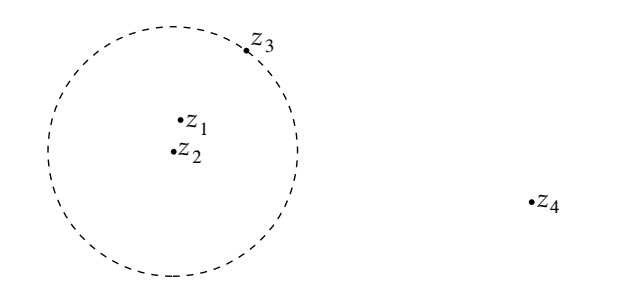
\includegraphics[width=0.8\textwidth,natwidth=400,natheight=180]{Fig2.1.jpg}\\
\caption{Expectation value of a product of four local operators. The OPE gives the asymptotics as $z_1 \to z_2$ as a series where the pair of operators at $z_1 $ and $ z_2$ is replaced by a single operator at $z_2$. The radius of convergence is the distance to	the nearest other operator, indicated by the dashed circle.}\label{Fig2.1}
	\end{center}
\end{figure}
上图是四个定域算符的乘积. OPE将$z_1 \to z_2$时渐近表示为一个级数. 其中$z_1 , z_2$一对算符被$z_2$处的单个算符代替. 收敛半径是到其他最近算符的距离.\\
OPE陈述为,两个彼此接近的定域算符的乘积可以以任意精度被定域算符的和近似:
\begin{equation}
\mathscr{A}_{i}\left(\sigma_{1}\right) \mathscr{A}_{j}\left(\sigma_{2}\right)=\sum_{k} c_{i j}^{k}\left(\sigma_{1}-\sigma_{2}\right) \mathscr{A}_{k}\left(\sigma_{2}\right)
\end{equation}
这是一个算符陈述,意味着其在一个普遍期望值中成立
\begin{equation}
\left\langle\mathscr{A}_{i}\left(\sigma_{1}\right) \mathscr{A}_{j}\left(\sigma_{2}\right) \ldots\right\rangle=\sum_{k} c_{i j}^{k}\left(\sigma_{1}-\sigma_{2}\right)\left\langle\mathscr{A}_{k}\left(\sigma_{2}\right) \ldots\right\rangle
\end{equation}
只要$\sigma_{1}$,$\sigma_{2}$之间的间隔小于与其他所有算符的距离.\\
系数函数 $c^{k}{ }_{i j}\left(\sigma_{1}-\sigma_{2}\right)$决定对间隔的依赖关系,其也依赖于i,j,k. 但与期望值中的其他算符无关. 后者的依赖性仅出现在(2.2.3)右边的期望值中. 这些项通常的排列方法是:$\sigma_{1} \rightarrow \sigma_{2}$的极限下,大小逐减. 这是对普通Taylor级数的类比. 除了系数函数不是简单的幂级数,并可以在$\sigma_{1} \rightarrow \sigma_{2}$时奇异.\\
我们现在将给出$X^\mu$理论的OPE推导. 其中利用了自由场论的特殊性质. 在2.9节将给出任意共形不变场论的推导. 我们已经看到,正规乘积满足运动方程(2.1.23). 这说明算符乘积是$\left(z_{1}, \bar{z}_{1}\right)$的调和函数. 复变函数论中一个简单的结果是,调和函数局域是一个全纯函数与一个反全纯函数之和. 尤其是,它意味着在$z_{1} \rightarrow z_{2}$时是不奇异的. 并且可以自由地以$z_{12}$ and $\bar{z}_{12}$ 做Taylor展开
\begin{equation}
\begin{array}{l}
X^{\mu}\left(z_{1}, \bar{z}_{1}\right) X^{v}\left(z_{2}, \bar{z}_{2}\right)=-\frac{\alpha^{\prime}}{2} \eta^{\mu \nu} \ln \left|z_{12}\right|^{2}+: X^{v} X^{\mu}\left(z_{2}, \bar{z}_{2}\right): \\
+\sum_{k=1}^{\infty} \frac{1}{k !}\left[\left(z_{12}\right)^{k}: X^{v} \partial^{k} X^{\mu}\left(z_{2}, \bar{z}_{2}\right):+\left(\bar{z}_{12}\right)^{k}: X^{v} \bar{\partial}^{k} X^{\mu}\left(z_{2}, \bar{z}_{2}\right):\right]
\end{array}
\end{equation}
\begin{remark}
$$\begin{aligned}
&:X^{\mu}\left(z_{1},  \bar{z}_{1}\right) X^{\nu}\left(z_{2}, \bar{z}_{2}\right):\\
=&: X^{\nu} X^{\mu}\left(z_{2}, \bar{z}_{2}\right):+\sum_{k=1}^{\infty} \frac{1}{k !}\left[\left(z_{12}\right)^{k}: X^{\nu} \partial^{k} X^{\mu}\left(z_{2}, \bar{z}_{2}\right):+\left(\bar{z}_{12}\right)^{k}:X^{\nu} \bar{\partial}^{k} X^{\mu}\left(z_{2}, \bar{z}_{2}\right):\right]
\end{aligned}
$$
倘若有定义
$$\partial_{1}:X^{\mu}\left(z_{1}, \bar{z}_{1}\right) X^{\nu}\left(z_{2}, \bar{z}_{2}\right):=: X^{\nu} \partial_{1}X^{\mu}:=X^{\nu} \partial_1 X^{\mu}+\frac{\alpha^{\prime}}{2} \eta^{\mu \nu} \partial_{1} \ln |z_{12}|^{2}$$
上式是可以解释的.
\end{remark}
------------------------------------------------------------------------------------------------------------
\\
Terms with mixed $\partial \bar{\partial}$ derivatives vanish by the equation of motion. This equation and many others simplify in units in which $\alpha^{\prime}=2$, which is the most common convention in the literature. However, several other conventions are also used, so it is useful to keep $\alpha^{\prime}$ explicit. For example, in open string theory equations simplify when $\alpha^{\prime}=\frac{1}{2}$.

Eq. (2.2.4) has the form of an OPE. Like the equation of motion ( $2.1 .23$ ) from which it was derived, it is an operator statement. For an arbitrary expectation value involving the product $X^{\mu}\left(z_{1}, \bar{z}_{1}\right) X^{v}\left(z_{2}, \bar{z}_{2}\right)$ times fields at other points, it gives the behavior for $z_{1} \rightarrow z_{2}$ as an infinite series, each term being a known function of $z_{12}$ and/or $\bar{z}_{12}$ times the expectation value with a local operator replacing the pair.

OPEs are usually used as asymptotic expansions, the first few terms
giving the dominant behavior at small separation. Most of our applications will be of this type, and we will often write OPEs as explicit singular
terms plus unspecified nonsingular remainders. The use of ‘∼’ in place of
‘=’ will mean ‘equal up to nonsingular terms.’ In fact, OPEs are actually
convergent in conformally invariant field theories. This will be very important to us in certain applications: it makes it possible to reconstruct
the entire theory from the coefficient functions. As an example, the freefield OPE (2.2.4) has a radius of convergence in any given expectation
value which is equal to the distance to the nearest other insertion in the
path integral. The operator product is harmonic except at the positions
of operators, and in particular inside the dashed circle of figure 2.1, and
convergence can then be shown by a standard argument from the theory
of complex variables.
The various operators on the right-hand side of the OPE (2.2.4) involve
products of fields at the same point. Usually in quantum field theory such
a product is divergent and must be appropriately cut off and renormalized,
but here the normal ordering renders it well-defined. Normal ordering is a
convenient way to define composite operators in free field theory. It is of
little use in most interacting field theories, because these have additional
divergences from interaction vertices approaching the composite operator
or one another. However, many of the field theories that we will be

interested in are free, and many others can be related to free field theories,
so it will be worthwhile to develop normal ordering somewhat further.
The definition of normal ordering for arbitrary numbers of fields can
be given recursively as
\begin{equation}
\begin{array}{l}
: X^{\mu_{1}}\left(z_{1}, \bar{z}_{1}\right) \ldots X^{\mu_{n}}\left(z_{n}, \bar{z}_{n}\right): \\
\quad=X^{\mu_{1}}\left(z_{1}, \bar{z}_{1}\right) \ldots X^{\mu_{n}}\left(z_{n}, \bar{z}_{n}\right)+\sum \text { subtractions }
\end{array}
\end{equation}
where the sum runs over all ways of choosing one, two, or more pairs of fields from the product and replacing each pair with $\frac{1}{2} \alpha^{\prime} \eta^{\mu_{i} \mu_{j}} \ln \left|z_{i j}\right|^{2}$. For example,\begin{equation}
\begin{array}{l}
: X^{\mu_{1}}\left(z_{1}, \bar{z}_{1}\right) X^{\mu_{2}}\left(z_{2}, \bar{z}_{2}\right) X^{\mu_{3}}\left(z_{3}, \bar{z}_{3}\right):=X^{\mu_{1}}\left(z_{1}, \bar{z}_{1}\right) X^{\mu_{2}}\left(z_{2}, \bar{z}_{2}\right) X^{\mu_{3}}\left(z_{3}, \bar{z}_{3}\right) \\
\quad+\left(\frac{\alpha^{\prime}}{2} \eta^{\mu_{1} \mu_{2}} \ln \left|z_{12}\right|^{2} X^{\mu_{3}}\left(z_{3}, \bar{z}_{3}\right)+2 \text { permutations }\right)
\end{array}
\end{equation}
We leave it to the reader to show that the definition (2.2.5) retains the desired property that the normal ordered product satisfies the naive equation
of motion.
The definition can be compactly summarized as
\begin{equation}
: \mathscr{F}:=\exp \left(\frac{\alpha^{\prime}}{4} \int d^{2} z_{1} d^{2} z_{2} \ln \left|z_{12}\right|^{2} \frac{\delta}{\delta X^{\mu}\left(z_{1}, \bar{z}_{1}\right)} \frac{\delta}{\delta X_{\mu}\left(z_{2}, \bar{z}_{2}\right)}\right) \mathscr{F}
\end{equation}
where $\mathscr{F}$ is any functional of $X .$ This is equivalent to eq. $(2.2 .5):$ the double derivative in the exponent contracts each pair of fields, and the exponential sums over any number of pairs with the factorial canceling the number of ways the derivatives can act. As an example of the use of this formal expression, act on both sides with the inverse exponential to obtain
\begin{equation}
\begin{aligned}
\mathscr{F} &=\exp \left(-\frac{\alpha^{\prime}}{4} \int d^{2} z_{1} d^{2} z_{2} \ln \left|z_{12}\right|^{2} \frac{\delta}{\delta X^{\mu}\left(z_{1}, \bar{z}_{1}\right)} \frac{\delta}{\delta X_{\mu}\left(z_{2}, \bar{z}_{2}\right)}\right): \mathscr{F}: \\
&=: \mathscr{F}:+\sum \text { contractions }
\end{aligned}
\end{equation}
where a contraction is the opposite of a subtraction: sum over all ways of choosing one, two, or more pairs of fields from $: \mathscr{F}:$ and replacing each pair with $-\frac{1}{2} \alpha^{\prime} \eta^{\mu_{i} \mu_{j}} \ln \left|z_{i j}\right|^{2}$.
The OPE for any pair of operators can be generated from
\begin{equation}
: \mathscr{F}:: \mathscr{G}:=: \mathscr{F} \mathscr{G}:+\sum \text { cross-contractions }
\end{equation}
for arbitrary functionals $\mathscr{F}$ and $\mathscr{G}$ of $X$. The sum now runs over all ways of contracting pairs with one field in $\mathscr{F}$ and one in $\mathscr{G} .$ This can also be written
\begin{equation}
: \mathscr{F}:: \mathscr{G}:=\exp \left(-\frac{\alpha^{\prime}}{2} \int d^{2} z_{1} d^{2} z_{2} \ln \left|z_{12}\right|^{2} \frac{\delta}{\delta X_{F}^{\mu}\left(z_{1}, \bar{z}_{1}\right)} \frac{\delta}{\delta X_{G \mu}\left(z_{2}, \bar{z}_{2}\right)}\right): \mathscr{F} \mathscr{G}:
\end{equation}
where the functional derivatives act only on the fields in $\mathscr{F}$ or $\mathscr{G}$ respectively. This follows readily from eq. (2.2.7). As an example,
\begin{equation}\label{2.2.11}
\begin{aligned}
&: \partial X^{\mu}(z) \partial X_{\mu}(z):: \partial^{\prime} X^{v}\left(z^{\prime}\right) \partial^{\prime} X_{v}\left(z^{\prime}\right): \\
=&: \partial X^{\mu}(z) \partial X_{\mu}(z) \partial^{\prime} X^{v}\left(z^{\prime}\right) \partial^{\prime} X_{v}\left(z^{\prime}\right): \\
&-4 \cdot \frac{\alpha^{\prime}}{2}\left(\partial \partial^{\prime} \ln \left|z-z^{\prime}\right|^{2}\right): \partial X^{\mu}(z) \partial^{\prime} X_{\mu}\left(z^{\prime}\right): \\
&+2 \cdot \eta^{\mu}{ }_{\mu}\left(-\frac{\alpha^{\prime}}{2} \partial \partial^{\prime} \ln \left|z-z^{\prime}\right|^{2}\right)^{2} \\
\sim &\frac{D \alpha^{\prime 2}}{2\left(z-z^{\prime}\right)^{4}}-\frac{2 \alpha^{\prime}}{\left(z-z^{\prime}\right)^{2}}: \partial^{\prime} X^{\mu}\left(z^{\prime}\right) \partial^{\prime} X_{\mu}\left(z^{\prime}\right): \\
&-\frac{2 \alpha^{\prime}}{z-z^{\prime}}: \partial^{\prime 2} X^{\mu}\left(z^{\prime}\right) \partial^{\prime} X_{\mu}\left(z^{\prime}\right):
\end{aligned}
\end{equation}
The second term in the equality comes from the four ways of forming a single pair and the third from the two ways of forming two pairs. In the final line we have put the OPE in standard form by Taylor expanding inside the normal ordering to express everything in terms of local operators at $z^{\prime}$ and putting the most singular terms first. \\
%$\underbracket{XYZUVW}$
%$\contraction{A}{B}{C}{D}ABCD$

\begin{remark}
$$
\begin{aligned}
&\contraction{: \partial}{X^{\mu}}{(z) \partial X_{\mu}(z):: \partial^{\prime}}{X^{\nu}}
: \partial  X^{\mu}(z) \partial X_{\mu}(z):: \partial^{\prime} X^{\nu} \left(z^{\prime}\right) \partial^{\prime} X_{\nu}\left(z^{\prime}\right):\\ =&\partial \partial^{\prime}\left(-\frac{\alpha^{\prime}}{2} \eta^{\mu \nu}|n| z-\left.z^{\prime}\right|^{2}\right): \partial X_{\mu}(z) \partial X_{\nu}(z):\\
=&-\left(\partial \partial^{\prime} \ln \left|z-z^{\prime}\right|^{2}\right) \cdot \frac{\alpha^{\prime}}{2}: \partial X_{\mu}(z) \partial^{\prime} X^{\mu}(z):
\end{aligned}
$$

$$
\begin{aligned}
&\contraction[2ex]{: \partial}{X^{\mu}}{(z) \partial X_{\mu}(z):: \partial^{\prime}}{X^{\nu}}
\bcontraction{: \partial X^\mu(z) \partial}{ X_\mu}{(z):: \partial^\prime X^\nu(z^\prime)\partial^\prime}{X_\nu}
	: \partial X^{\mu}(z) \partial X_{\mu}(z):: \partial^{\prime} X^{\nu}\left(z^{\prime}\right) \partial^{\prime} X_{\nu}\left(z^{\prime}\right):\\
=&\partial \partial^{\prime}\left(-\frac{\alpha^{\prime}}{2} \eta ^{\mu \nu} \ln \left|z-z^{\prime}\right|^{2}\right) \partial \partial^{\prime}\left(-\frac{\alpha^{\prime}}{2} \eta^{\mu \nu}\ln \left|z-z^{\prime}\right|^{2}\right) \\
=&\eta^{\mu \nu} \eta_{\mu \nu}\left(-\frac{\alpha^{\prime}}{2} \partial \partial^{\prime}\ln | z-\left.z^{\prime}\right|^{2}\right)^{2}
\end{aligned}
$$
而
$\eta^{\mu \nu} \eta_{\nu\rho}=\delta^{\mu}{ }_{p}, \quad \eta^{\mu \nu} \eta_{\mu \nu}=\delta^{\mu}{ }_{\mu}=D$,
且
$$
(1)=2 \cdot \eta^{\mu}{ }_{\mu}\left(-\frac{\alpha^{\prime}}{2} \frac{1}{\left(z-z^{\prime}\right)^{2}}\right)^{2}=2 D \cdot \frac{\alpha^{\prime 2}}{4} \frac{1}{\left(z-z^{\prime}\right)^{4}}=\frac{D \alpha^{\prime 2}}{2\left(z-z^{\prime}\right)^{4}}
$$

$$
(2)=\partial \partial^{\prime} \ln \left|z-z^{\prime 2}\right|^{2}=\partial \partial^{\prime}\left(\ln \left(z-z^{\prime}\right)+\ln \left(\bar{z}+\bar{z}^{\prime}\right)=\partial^{\prime} \frac{1}{z-z^{\prime}}=+\frac{1}{\left(z^{\prime}-z\right)^{2}}\right.
$$

$$
(3)=:\partial X^\mu(z)\partial^\prime X_{\mu}(z^\prime):\sim \partial^\prime X^\mu(z^\prime)\partial^\prime X_\mu(z^\prime): +(z-z^\prime):\partial^{\prime 2} X^\mu(z^\prime)\partial^\prime X_\mu(z):
$$
于是
$$
: \partial X^{\mu}(z) \partial X_{\mu}(z):: \partial^{\prime} X^{\nu}\left(z^{\prime}\right) \partial^{\prime} X_{\nu}\left(z^{\prime}\right):  \sim (1)+(2)\cdot(3)
$$
\end{remark}
Another important example is
\begin{equation}
\mathscr{F}=e^{i k_{1} \cdot X(z, \bar{z})}, \quad \mathscr{G}=e^{i k_{2} \cdot X(0,0)}
\end{equation}
The variations $\delta / \delta X_{F}^{\mu}$ and $\delta / \delta X_{G}^{\mu}$ give factors of $i k_{1 \mu}$ and $i k_{2 \mu}$ respectively, so the general result $(2.2 .10)$ becomes
\begin{equation}\label{2.2.13}
\begin{aligned}
: e^{i k_{1} \cdot X(z, \bar{z})}:: e^{i k_{2} \cdot X(0,0)}: &=\exp \left(\frac{\alpha^{\prime}}{2} k_{1} \cdot k_{2} \ln |z|^{2}\right): e^{i k_{1} \cdot X(z, \bar{z})} e^{i k_{2} \cdot X(0,0)} :\\
&=|z|^{\alpha^{\prime} k_{1} \cdot k_{2}}: e^{i k_{1} \cdot X(z, \bar{z})} e^{i k_{2} \cdot X(0,0)}:
\end{aligned}
\end{equation}

\begin{remark}
$$
\begin{aligned}
&:e^{i k_{1} \cdot x(z, z)}:: e^{i k_{2} \cdot x(0.0)}:\\
=&\exp \left(-\frac{\alpha^{\prime}}{2} \int d^{2} z_{1} d^{2} z_{2} \ln \left|z_{12}\right|^{2} \frac{\delta}{\delta X_{F}^{\mu}\left(z_{1}, \bar{z}_{1}\right)} \frac{\delta}{\delta X_{G\mu}\left(z_{2}, \bar{z}_{2}\right)}\right): e^{i k_{1} \cdot x(z, \bar{z})} e^{i k_{2} \cdot x(0,0)}:\\
=&\left(1-\frac{\alpha^{\prime}}{2} \int d^{2} z_{1} d^{2} z_{2} \ln \left|z_{12}\right|^{2} \frac{\delta}{\delta X_{F}^{\mu}\left(z_{1}, z_{1}\right)} \frac{\delta}{\delta X_{G \mu}\left(z_{2}, \bar{z}_{2}\right)} \right): e^{i k_{1} \cdot x(z, \bar{z})} e^{i k_{2} \cdot x(0,0)}:+\cdots\\
=&: e^{i k_{1} \cdot x(z, \bar{z})} e^{i k_{2} \cdot x(0,0)}-\frac{\alpha^{\prime}}{2} \int d^{2} z_{1} d^{2} z_{2} \ln \left|z_{12}\right|^{2}
:e^{i k_{1} \cdot x\left(z, \bar{z}\right)} e^{i k_{2} \cdot x ( 0,0)}:\\
&\qquad \qquad \qquad \qquad \qquad
 \times i k_{1 \mu} \delta\left(z-z_{1}, \bar{z}-\bar{z}_{1}\right) i k_{2}^{\mu} \delta\left(0-z_{2}, 0,-\bar{z}_{2}\right)\\
=&e^{i k_{1} \cdot x(z, \bar{z})} e^{i k_{2} \cdot x(0,0)}:\left(1+\frac{\alpha^{\prime}}{2} k_{1} \cdot k_{2} \ln |z|^{2}+\cdots\right)
\end{aligned}
$$
\end{remark}

To derive the OPE, Taylor expand inside the normal ordering to give
\begin{equation}
: e^{i k_{1} \cdot X(z, \bar{z})}:: e^{i k_{2} \cdot X(0,0)}:=|z|^{\alpha^{\prime} k_{1} \cdot k_{2}}: e^{i\left(k_{1}+k_{2}\right) \cdot X(0,0)}[1+O(z, \bar{z})]:
\end{equation}
The exercises give further practice with normal ordering and the free-field OPE.

Note that the OPEs (2.2.2), (2.2.4), and so on have been written asymmetrically in $\sigma_{1}$ and $\sigma_{2}$, expanding around the latter point. They can also be cast in symmetric form by Taylor expanding the right-hand sides around $\left(\sigma_{1}+\sigma_{2}\right) / 2$. The coefficient functions for the symmetric form behave simply under interchange of the two operators,
\begin{equation}
c_{i j}^{k}\left(\sigma_{1}-\sigma_{2}\right)_{\mathrm{sym}}=\pm c_{j i}^{k}\left(\sigma_{2}-\sigma_{1}\right)_{\mathrm{sym}}
\end{equation}
where the minus sign appears if $\mathscr{A}_{i}$ and $\mathscr{A}_{j}$ are both anticommuting. The asymmetric form is usually more convenient for calculation, so when the
symmetry properties of the coefficient functions are needed one can work
them out in the symmetric form and then convert to the asymmetric form.

\section{Ward恒等式}%{2.3 Ward identities and Noether theorem}
世界面对称性在弦论中扮演了一个重要角色. 在本节,我们先导出场论中对称性的一些普遍结果.\\
考察一个场论,作用量为$S_\phi$. 在d维时空中,$\phi_\alpha(\sigma)$标记一般场. 让它存在对称性
\begin{equation}
\phi_{\alpha}^{\prime}(\sigma)=\phi_{\alpha}(\sigma)+\delta \phi_{\alpha}(\sigma)
\end{equation}
其中$\delta \phi_\alpha$正比于无限小参量$\epsilon$. 路径积分测度与权重$exp(-S)$之积是不变的:
\begin{equation}
\left[d \phi^{\prime}\right] \exp \left(-S\left[\phi^{\prime}\right]\right)=[d \phi] \exp (-S[\phi])
\end{equation}
场论中,连续对称性暗示着守恒流的存在(Noether定理),以及Ward等式(其约束流的算符积). 为了导出这些结果,考察变量的改变
\begin{equation}\label{2.3.3}
\phi_{\alpha}^{\prime}(\sigma)=\phi_{\alpha}(\sigma)+\rho(\sigma) \delta \phi_{\alpha}(\sigma)
\end{equation}
这不是对称性,$[\dif \phi]\mathrm{exp}(-S)$在$\rho$是一常量下不变,所以它的变分必须正比于$\partial _a \rho$
\begin{equation}
\begin{array}{l}
{\left[d \phi^{\prime}\right] \exp \left(-S\left[\phi^{\prime}\right]\right)} \\
\quad=[d \phi] \exp (-S[\phi])\left[1+\frac{i \epsilon}{2 \pi} \int d^{d} \sigma g^{1 / 2} j^{a}(\sigma) \partial_{a} \rho(\sigma)+O\left(\epsilon^{2}\right)\right]
\end{array}
\end{equation}
未知系数$j^a(\sigma)$源于测度和作用量的变分,仅在一个小区域里取$\rho$非零. 在区域之外,考察一个普遍插入$'\cdots'$ 的路径积分。这个插入(\ref{2.3.3}) 下不变:
\begin{equation}
\begin{aligned}
0 &=\int\left[d \phi^{\prime}\right] \exp \left(-S\left[\phi^{\prime}\right]\right) \ldots-\int[d \phi] \exp (-S[\phi]) \ldots \\
&=\frac{\epsilon}{2 \pi i} \int d^{d} \sigma g^{1 / 2} \rho(\sigma)\left\langle\nabla_{a} j^{a}(\sigma) \ldots\right\rangle
\end{aligned}
\end{equation}
因而我们有
\begin{equation}
\nabla_{a} j^{a}=0
\end{equation}

\begin{remark}
(2.3.4)的补充说明:
$$
\frac{i \epsilon}{2 \pi} \int d ^d \sigma g^{1 / 2} j^{a}(\sigma) \partial_{a} \rho(\sigma) 
=\frac{\epsilon}{2 \pi i} \int d^{d} \sigma \partial_{a}\left(g^{1 / 2}j^{a}\right)\rho(\sigma)
$$
$$
\partial_{a}\left(g^{1 / 2} j^{a}\right)=\partial_{a} j^{a} \cdot g^{1 / 2}+j^{a} \partial_{a} g^{1 / 2}
=g^{1 / 2}\nabla_{a}j^{a}
$$
\end{remark}
为了导出ward等式,令$\rho(\sigma)$在区域R内为1,在R外为0. 另外在路径积分中引入一般定域算符$\mathscr{A}\left(\sigma_{0}\right)$. $\sigma_0$在R内. 在R外引入$'\cdots'$得到
\begin{equation}
\delta \mathscr{A}\left(\sigma_{0}\right)+\frac{\epsilon}{2 \pi i} \int_{R} d^{d} \sigma g^{1 / 2} \nabla_{a} j^{a}(\sigma) \mathscr{A}\left(\sigma_{0}\right)=0
\end{equation}

\begin{proof}
关于(2.3.7)的证明:
由(2.3.4)
$$
\delta \exp \left(-S\left[\phi^{\prime}\right]\right)=\frac{ \epsilon}{2 \pi i} \int d^{d} \sigma g^{1 / 2} \nabla_{a} j^{a}(\sigma) \rho(\sigma) \cdot e^{-S}
$$
$$
\delta\left[\exp (-S[\phi]) \mathscr{A}\left(\sigma_{0}\right)\right]=\delta e^{-S} \mathscr{A}\left(\sigma_{0}\right)+e^{-S} \delta\mathscr{A}(\sigma_0)=0
$$
$$
\delta \mathscr{A}\left(\sigma_{0}\right) +\mathscr{A}\left(\sigma_{0}\right) e^{S} \delta e^{-S}=0
$$
$$
\delta \mathscr{A}\left(\sigma_{0}\right)+\frac{\sigma}{2 \pi i} \int_{R} d^{d} \sigma g^{1 / 2} \nabla_{a} j^{a}(\sigma) \mathscr{A}\left(\sigma_{0}\right)=0
$$
而
$$
\int_{R} d^{d} \sigma g^{1 / 2} \nabla_{a} j^{a} =\int_{R} d^{d} \sigma \partial_{a}\left(g^{1 / 2} j^{a}\right) 
=\int_{\partial R} d A n_{\alpha} j^{a}
$$
在复坐标下
$$
\int_{R} d^{2} z\left(\partial_{z} v^{z}+\partial_{\bar{z}} v^{\bar{z}}\right)=i \oint_{\partial R}(v^{z} d \bar{z}-v^{\bar{z}} d \bar{z})
$$
$$
\int g^{1 / 2} \nabla_{a} j^{a}=\int\left(\partial_{z} j^{z}+\partial_{\bar{z}} j^{\bar{z}}\right)\frac{1}{2}=\int 2\left(\partial_{z} j_{\bar{z}}+\partial_{z} j_{z}\right) \frac{1}{2}
$$
\end{proof}

等价地,
\begin{equation}
\nabla_{a} j^{a}(\sigma) \mathscr{A}\left(\sigma_{0}\right)=g^{-1 / 2} \delta^{d}\left(\sigma-\sigma_{0}\right) \frac{2 \pi}{i \epsilon} \delta \mathscr{A}\left(\sigma_{0}\right)+\text { total } \sigma \text { -derivative }
\end{equation}
散度定理给出
\begin{equation}
\int_{\partial R} d A n_{a} j^{a} \mathscr{A}\left(\sigma_{0}\right)=\frac{2 \pi}{i \epsilon} \delta \mathscr{A}\left(\sigma_{0}\right)
\end{equation}
在2维平坦空间中
\begin{equation}
\oint_{\partial R}(j d z-\tilde{\jmath} d \bar{z}) \mathscr{A}\left(z_{0}, \bar{z}_{0}\right)=\frac{2 \pi}{\epsilon} \delta \mathscr{A}\left(z_{0}, \bar{z}_{0}\right)
\end{equation}
在这里我们扔掉了指标$j \equiv j_{z}, \tilde{\jmath} \equiv j_{\bar{z}}$. 我们使用$\tilde{j}$而非$\bar{j}$是因为$\tilde{j}$并非j的共轭. Minkowski密度$j_0$一般是Hermitean的,$\left(j_{z}\right)^{\dagger}=\frac{1}{2}\left(j_{1}-i j_{2}\right)^{\dagger}=j_{z}$.\\
重要的是Noether定理和Ward等式是定域性质,并不依赖于远处的边界条件,也不依赖在对称下是否不变. 特别的,因为$\rho(\sigma)$仅在R内非零,仅需要在这里定义对称变换.\\
在共形不变理论中,通常$j_z$是全纯的,而$j_{\bar{z}}$是反全纯的. 在这种情况下,流$(j_z,0),(0,j_{\bar{z}})$分别守恒. 于是积分给出OPE中的留数:
\begin{equation}\label{2.3.11}
\operatorname{Res}_{z \rightarrow z_{0}} j(z) \mathscr{A}\left(z_{0}, \bar{z}_{0}\right)+\overline{\operatorname{Res}}_{\bar{z} \rightarrow \bar{z}_{0}} \tilde{J}(\bar{z}) \mathscr{A}\left(z_{0}, \bar{z}_{0}\right)=\frac{1}{i \epsilon} \delta \mathscr{A}\left(z_{0}, \bar{z}_{0}\right)
\end{equation}
这里$\mathrm{Res},\mathrm{\bar{Res}}$分别是$\left(z-z_{0}\right)^{-1}, \left(\bar{z}-\bar{z}_{0}\right)^{-1}$的系数.\\
一个例子:无质量自由标量场\\
考虑时空平移$\delta X^{\mu}=\epsilon a^{\mu}$. 在$\delta X^{\mu}(\sigma)=\epsilon \rho(\sigma) a^{\mu}$ 下,
\begin{equation}
\begin{aligned}
\delta S&=\frac{1}{4 \pi \alpha^{\prime}} \int d^{2} \pm 2 \delta \partial^{a} X^{\mu} \partial_{a} X_{\mu}\\
&=-\frac{1}{2\pi \alpha^{\prime}} \int d^{2} z \delta X^{\mu} \partial^{a} \partial_{a} X_{\mu} \\
&=-\frac{1}{2 \pi \alpha^{\prime}} \int d^{2} z \quad \epsilon p(\sigma) a^{\mu} \partial^{a} \partial_{a} X_{\mu}\\
&=\frac{\epsilon a_{\mu}}{2 \pi \alpha^{\prime}} \int d^{2} \sigma \partial^{a} X^{\mu} \partial_{a} \rho
\end{aligned}
\end{equation}
令$\delta S=\frac{i \epsilon}{2 \pi \alpha^\prime} \int d^{2} z \, j^{a}(\sigma)  \partial _a \rho$,则
$j_{a}(\sigma)=a_{\mu} j_{a}^{\mu}$
\begin{equation}
j_{a}^{\mu}=\frac{i}{\alpha^{\prime}} \partial_{a} X^{\mu}
\end{equation}
并且
\begin{subequations}
\begin{equation}
j^{\mu}(z): e^{i k \cdot X(0,0)}: \sim \frac{k^{\mu}}{2 z}: e^{i k \cdot X(0,0)}:
\end{equation}
\begin{equation}
\tilde{\jmath}^{\mu}(\bar{z}): e^{i k \cdot X(0,0)}: \sim \frac{k^{\mu}}{2 \bar{z}}: e^{i k \cdot X(0,0)}:
\end{equation}
\end{subequations}

\begin{proof}
(2.3.14a)的说明:
由(2.3.13)
$$
j^{\mu}=j_{z}^{\mu}=\frac{i}{\alpha^{\prime}} \partial_{z} X^{\mu}
$$
$$
\begin{aligned}
& \frac{i}{\alpha^{\prime}}: \partial_{z}X^{\mu}: : e^{i k \cdot x(0,0)}: \\
=& \frac{i}{\alpha^{\prime}} \exp \left(-\frac{\alpha^{\prime}}{2} \int d^{2} z_{1} d^{2} z_{2} \ln \left|z_{12}\right|^{2} \frac{\delta}{\delta X_{F}^{\mu}\left(z_{1}, \bar{z}_{1}\right)} \frac{\delta}{\delta X_{G{\mu}}\left(z_{2}, \bar{z}_{2}\right)}\right): \partial_{z}X^{\mu} e^{i k \cdot x(0,0)}: \\
=& \frac{i}{\alpha^{\prime}}\left(1-\frac{\alpha^{\prime}}{2} \int d^{2} z_{1} d^{2} z_{2} \ln \left|z_{12}\right|^{2} \frac{\delta}{\delta X^{\mu}} \frac{\delta}{\delta X_{u}}-\cdots\right) : \partial_{z} X^{\mu} e^{i k \cdot x}:\\
=&\frac{i}{\alpha^{\prime}}: \partial_{z} X^{\mu} e^{i k  x(0,0)}:-\frac{i}{2} \partial_{z} \int d^{2} z_{1} d^{2} z_{2} \ln \left|z_{12}\right|^{2} \delta\left(z-z_{1}, \bar{z}-\bar{z}_{1}\right)  i k_{2}^{\mu} \delta\left(-z_{2}, -\bar{z}_{2}\right):e^{ikx}:\\
\sim&-\frac{i}{2} \partial_{z} \ln |z|^{2} \cdot i k^{\mu}: e^{i k \cdot x(0,0)}: \\
=&\frac{1}{2} \frac{1}{z} i k^{\mu}: e^{i k \cdot x(0,0)}:=\frac{i k^{\mu}}{2 z}: e^{i k \cdot x(0,0)}:
\end{aligned}
$$
\end{proof}

另一例子:世界面平移$\delta \sigma^{a}=\epsilon v^{a}$\\
这时$\delta X^{\mu}=-\epsilon v^{a} \partial_{a} X^{\mu}$,Noether流
\begin{subequations}
\begin{equation}\label{2.3.15a}
j_{a}=i v^{b} T_{a b}
\end{equation}
\begin{equation}
T_{a b}=-\frac{1}{\alpha^{\prime}}:\left(\partial_{a} X^{\mu} \partial_{b} X_{\mu}-\frac{1}{2} \delta_{a b} \partial_{c} X^{\mu} \partial^{c} X_{\mu}\right):
\end{equation}
\end{subequations}

\begin{proof}
(2.3.15a)的证明:
$$
\delta \sigma^{u}=\epsilon v^{a}, \quad \delta X^{\mu}=-\partial_{a} X^{\mu} \delta \sigma^{a}=-\epsilon v^{a} \partial_{a} X^{\mu}
$$
$$
\begin{aligned}
\delta S &=\frac{1}{4 \pi \alpha^{\prime}} \int d^{2} \sigma 2 \delta \partial^{\alpha} X^{\mu} \partial_{a} X_{\mu} \\
&=-\frac{1}{2 \pi \alpha^{\prime}} \int d^{2} \sigma \delta X^{\mu} \partial^{a} \partial_{a} X_{\mu} \\
&=-\frac{1}{2 \pi \alpha^{\prime}} \int d^{2} \sigma\left(-\epsilon v^{a} \partial_{\alpha} X^{\mu}\right) \rho(\sigma) \partial^{\alpha} \partial_{a} X_{\mu} \\
&=\frac{\epsilon v^{\alpha}}{2 \pi \alpha^{\prime}} \int d^{2} \sigma  \partial_{a} X^{\mu} \rho(\sigma) \partial^{b} \partial_{b} X_{u}
\end{aligned}
$$
$$
\begin{array}{l}
\int d^{2} \sigma \partial_{b}\left(\partial_{a} X^{\mu} \rho(\sigma)\right) \partial^{b} X_{u} \\
=\int d^{2} \sigma  \partial_{a} X^{\mu} \partial^{b} X_{\mu} \partial_{b} \rho(\sigma)+\rho(\sigma) \partial_{b} \partial_{a} X^{\mu} \partial^{b} X_{\mu}\\
=\int d^{2} \sigma \partial_{a} X^{\mu} \partial^{b} X_{\mu} \partial_{b} \rho(\sigma)-\partial_{a} \rho(\sigma) \partial_{b} X^{\mu} \partial^{b} X_{\mu}-\rho(\sigma) \partial_{a} X^{\mu} \partial_{b} \partial^{b} X^{\mu} \\
=\int d^{2} \sigma \partial_{a} X^{\mu} \rho(\sigma) \partial^{b} \partial_{b} X^{\mu} \\
=\frac{1}{2} \int d^{2} \sigma \partial_{a} X^{\mu} \partial^{b} X_{\mu} \partial_{b} \rho(\sigma)-\partial_{a} \rho(\sigma) \partial_{b} X^{\mu} \partial^{b} X_{u}
\end{array}
$$
$$
\frac{\epsilon v^{a}}{2 \pi \alpha^{\prime}} \int d^{2} \sigma \frac{1}{2} \left[\partial_{a} X^{\mu} \partial^{b} X_{\mu} \partial_{b} \rho(\sigma)-\partial_{a}\rho \partial_{b} X^{\mu}  \partial^{b} X_{\mu}\right]=\frac{i \epsilon}{2 \pi} \int d^{2} z j^{a}(\sigma) \partial_{a}(\rho)
$$
\end{proof}


\section{共形不变性}%{2.4 Conformal invariance}

能动量张量(\ref{2.3.15a})是无迹的,${T_a} ^a=0$. 在复坐标中,则是
\begin{equation}
T_{z \bar{z}}=0
\end{equation}
守恒律$\partial^a T_{ab}=0$暗示着在任何${T_a} ^a=0$的理论中
\begin{equation}
\bar{\partial} T_{z z}=\partial T_{\bar{z} \bar{z}}=0
\end{equation}
因此
\begin{equation}
T(z) \equiv T_{z z}(z), \quad \tilde{T}(\bar{z}) \equiv T_{\bar{z} \bar{z}}(\bar{z})
\end{equation}
分别是全纯的和反全纯的. 对于无质量自由标量
\begin{equation}\label{2.4.4}
T(z)=-\frac{1}{\alpha^{\prime}}: \partial X^{\mu} \partial X_{\mu}:, \quad \tilde{T}(\bar{z})=-\frac{1}{\alpha^{\prime}}: \bar{\partial} X^{\mu} \bar{\partial} X_{\mu}:
\end{equation}
作为运动方程的结果,其确实是全纯和反全纯的.\\
$T_{ab}$的无迹暗示着一个大得多的对称性. 流
\begin{equation}
j(z)=i v(z) T(z), \quad \tilde{\jmath}(\bar{z})=i v(z)^{*} \tilde{T}(\bar{z})
\end{equation}
对于全纯的$v(z)$是守恒的.
\begin{proof}
$$
j_{z}=i v^{z} T_{z z}, \quad j_{\bar{z}}=i v^{\bar{z}} T_{\bar{z} \bar{z}}
$$
由(2.1.5)
$$
v^{z}={v^{\bar{z}}}^*
$$
而
$$
\nabla_{a} j^{a}= \bar{\partial} j_{z}+\partial j_{\bar{z}}=0
$$
所以$v^z$为全纯.
\end{proof}
对于自由标量理论,得到OPE
\begin{equation}
T(z) X^{\mu}(0) \sim \frac{1}{z} \partial X^{\mu}(0), \quad \tilde{T}(\bar{z}) X^{\mu}(0) \sim \frac{1}{\bar{z}} \bar{\partial} X^{\mu}(0)
\end{equation}
\begin{proof}
$$
T(z)=-\frac{1}{\alpha^{\prime}}: \partial X^{\mu} \partial X_{\mu}:
$$
$$
-\frac{1}{\alpha^{\prime}}: \partial X^{\mu} \partial X_{\mu}: X^{\nu}(0)=-\frac{1}{\alpha^{\prime}}: \partial X^{\mu} \partial X_{\mu}(z) X^{\nu}(0):\sim \frac{1}{z} \partial X_{\mu} (0)
$$
\end{proof}
那么Ward等式给出变换
\begin{equation}\label{2.4.7}
\delta X^{\mu}=-\epsilon v(z) \partial X^{\mu}-\epsilon v(z)^{*} \bar{\partial} X^{\mu}
\end{equation}
\begin{proof}
由(\ref{2.3.11})
$$
\frac{1}{i \epsilon} \delta X^{\mu}=\operatorname{Res}_{z \rightarrow z_{0}^{\prime}} i v^{z} T_{z z} X^{\mu}+\overline{\operatorname{Res}}_{z \rightarrow z_{0}} i v^{\bar{z}} T_{\bar{z} \bar{z}} X^{\mu}
$$
前者$=i v^{z} \frac{1}{z-z_0} \partial X^{\mu}\left(z_{0}\right)$,
后者$=i v^{z *} \frac{1}{z} \bar{\partial} X^{\mu}\left(z_{0}\right)$
$$
\delta X^{\mu}=-\epsilon v^{z} \partial X^{\mu}\left(z_{0}\right)-\epsilon v^{\bar{z}} \bar{\partial} X^{\mu}\left(\bar{z}_{0}\right)
$$
\end{proof}
这是无限小坐标变换$z^{\prime}=z+\epsilon v(z)$. 
有限变换
\begin{equation}
X^{\prime \mu}\left(z^{\prime}, \bar{z}^{\prime}\right)=X^{\mu}(z, \bar{z}), \quad z^{\prime}=f(z)
\end{equation}
这是共形变换.
共形不变不应与diff不变相混淆. 我们处在平坦空间中,没有独立的度规场以供变化. 所以变换$z\to z^\prime$真的改变了内点的距离. 我们不是随随便便就有了这种不变性,它是关于动力学的非平庸陈述. 对于标量作用量(2.1.10),$\partial,\bar{\partial}$的共形变换与$d^2 z$的共形变换恰好抵消,质量项$m^{2} X^{\mu} X_{\mu}$将是不变的.
最终,存在一个与Polyakov弦的$diff\times Weyl$对称性的紧密联系. \\
考察特殊情况
\begin{equation}\label{2.4.9}
z^{\prime}=\zeta z
\end{equation}
$\zeta$为任意复数. $\zeta$的相位是系统的旋转,它的大小则是系统尺寸的重新标度. 这种标度不变性通常视为粒子物理中的一个近似对称性以及被标度不变场论描述的统计系统在临界点附近所拥有的近似对称性. \\
对于广义共形变换,考察$d s^{2}=d \sigma^{a} d \sigma^{a}=d z d \bar{z}$ 上的效应
\begin{equation}
d s^{\prime 2}=d z^{\prime} d \bar{z}^{\prime}=\frac{\partial z^{\prime}}{\partial z} \frac{\partial \bar{z}^{\prime}}{\partial \bar{z}} d z d \bar{z}
\end{equation}
我们看到共形变换将无限小平方变为无限小平方并调节了大小. 一个反全纯函数$z^{\prime}=f(z)^{*}$ 有相同的性质但改变了方向. \\
在(\ref{2.4.9})下不变的大多数系统通常在大得多的共形不变性不变. 有这种不变性的理论称为共形场论(CFT). \\
\begin{figure}
	\begin{center}
		%	\includegraphics[width=0.8\textwidth,bb=0 0 803 312]{Fig2.3ClosedStringCoordinates.jpg}\\
		%1px=0.75pt
		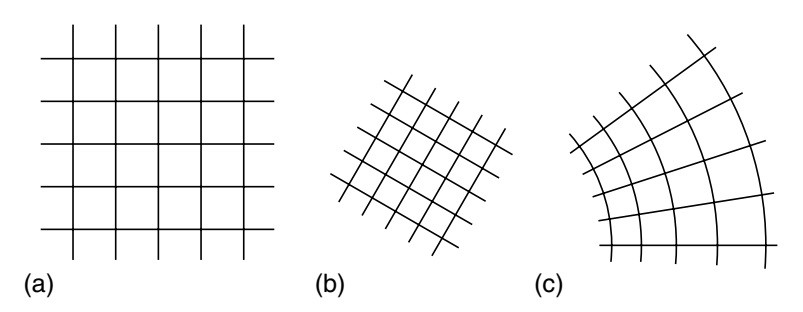
\includegraphics[width=0.8\textwidth,natwidth=520,natheight=200]{Fig2.2.jpg}\\
\caption{(a) Two-dimensional region. (b) Effect of the special conformal transformation (2.4.9). (c) Effect of a more general conformal transformation.}
	\end{center}
\end{figure}

\centerline{\Large 共形不变与OPE}
共形不变给OPE的形式施加了一个很强的约束,尤其是能动量张量的OPE. 考察T与一般算符$\mathscr{A}$的OPE. 因为$T(z)$和 $\tilde{T}(\bar{z})$除了交叉点以外是(反)全纯的,相应的系数函数也要有这个性质. T与$\mathscr{A}$的OPE因而是Laurent展开,是z的整数次但可能为负幂级数. 更进一步,所有项都由$\mathscr{A}$的共形变换决定. 为了看到这一点,我们写出一奇异性的普遍展开
\begin{equation}\label{2.4.11}
T(z) \mathscr{A}(0,0) \sim \sum_{n=0}^{\infty} \frac{1}{z^{n+1}} \mathscr{A}^{(n)}(0,0)
\end{equation}
与$\tilde{T}$相似,算符系数$\mathscr{A}^{(n)}$留到以后决定. 在无限小共形变换$z^{\prime}=z+\epsilon v(z)$下,当$T \mathscr{A}$ OPE中的$z^{-n-1}$ 项与$v(z)$中 $z^n$项相乘时,在$v(z) T(z) \mathscr{A}(0,0)$ 中会出现一个单极点. 
因此Ward等式的(\ref{2.3.11})形式暗示
\begin{equation}\label{2.4.12}
\delta \mathscr{A}(z, \bar{z})=-\epsilon \sum_{n=0}^{\infty} \frac{1}{n !}\left[\partial^{n} v(z) \mathscr{A}^{(n)}(z, \bar{z})+\bar{\partial}^{n} v(z)^{*} \tilde{\mathscr{A}}^{(n)}(z, \bar{z})\right]
\end{equation}
因此算符$\mathscr{A}^{(n)}$ 由$\mathscr{A}$的共形变换决定. 取在刚性变换(\ref{2.4.9})下为本征态的算符为基是方便的
\begin{equation}\label{2.4.13}
\mathscr{A}^{\prime}\left(z^{\prime}, \bar{z}^{\prime}\right)=\zeta^{-h \bar{\zeta}-\tilde{h}} \mathscr{A}(z, \bar{z})
\end{equation}
$(h, \tilde{h})$称为权重. $h+ \tilde{h}$是$\mathscr{A}$的维数,决定了$\mathscr{A}$在重新标度下的行为,而$h- \tilde{h}$是自旋,决定它在旋转下的行为. 导数$\partial_z$ 提升 $h$ 一次,  $\partial_{\bar{z}}$ 提升 $\tilde{h}$ 一次. 变换(\ref{2.4.13})的Ward等式与平移$\delta \mathscr{A}=-\epsilon v^{a} \partial_{a} \mathscr{A}$ 的Ward等式决定了OPE的部分
\begin{equation}\label{2.4.14}
T(z) \mathscr{A}(0,0)=\ldots+\frac{h}{z^{2}} \mathscr{A}(0,0)+\frac{1}{z} \partial \mathscr{A}(0,0)+\ldots
\end{equation}
对$\tilde{T}$类似.\\
\begin{remark}
变换(\ref{2.4.13})造成的偏移是
$$
\begin{aligned}
\delta \mathscr{A} &=\mathscr{A}^{\prime}(z, \bar{z})-\mathscr{A}(z, \bar{z}) \\
&=\mathscr{A}^{\prime}(z^{\prime} / \zeta, \bar{z}^{\prime} / \zeta)-\mathscr{A} ( z, \bar{z})
\end{aligned}
$$
令$\zeta=1+\epsilon v, \quad z^{\prime} / (1+\epsilon v)=z^{\prime}(1-\epsilon v)$
则
$$
\begin{aligned}
\delta \mathscr{A} &=\mathscr{A}^{\prime}(z^{\prime}, \bar{z}^{\prime})-\epsilon v z^{\prime} \partial \mathscr{A}^{\prime}\left(z^{\prime}\right)-\epsilon \bar{v}{\bar{z}^{\prime}} \bar{\partial} \mathscr{A}^{\prime}(\bar{z}^{\prime})-\mathscr{A}(z, z^{\prime}) \\
&=[(1+\epsilon v)^{h}(1+\epsilon v)^{-h} \mathscr{A}-1]   \mathscr{A}(z, z^{\prime}) 
-\epsilon v z^{\prime} \partial \mathscr{A}^{\prime}(z^{\prime})-\epsilon \bar{v} \bar{z}^{\prime} \bar{\partial} \mathscr{A}^{\prime}(\bar{z}^{\prime})
\end{aligned}
$$
\end{remark}
一个特别重要的是张量算符或基础场$\mathcal{O}$.  一个一般共形变换作用其上为
\begin{equation}
\mathcal{O}^{\prime}\left(z^{\prime}, \bar{z}^{\prime}\right)=\left(\partial_{z} z^{\prime}\right)^{-h}\left(\partial_{\bar{z}} \bar{z}^{\prime}\right)^{-\tilde{h}} \mathcal{O}(z, \bar{z})
\end{equation}
OPE(\ref{2.4.11})约化成
\begin{equation}\label{2.4.16}
T(z) \mathcal{O}(0,0)=\frac{h}{z^{2}} \mathcal{O}(0,0)+\frac{1}{z} \partial \mathcal{O}(0,0)+\ldots
\end{equation}
普遍OPE(\ref{2.4.14})中更加奇异的项没有了.\\
再取一次自由$X^\mu$CFT 的例子. 某些典型算符的权重是
\begin{equation}
\left.\begin{array}{llll}
X^{\mu} & (0,0), & \partial X^{\mu} & (1,0) \\
\bar{\partial} X^{\mu} & (0,1), & \partial^{2} X^{\mu} & (2,0) \\
: e^{i k \cdot X}: & \left(\frac{\alpha^{\prime} k^{2}}{4}, \frac{\alpha^{\prime} k^{2}}{4}\right) & &
\end{array}\right\}
\end{equation}
除了$\partial^{2} X^{\mu}$,所有量都按张量变换. 更一般地,指数与导数的一般乘积
\begin{equation}
:\left(\prod_{i} \partial^{m_{i}} X^{\mu_{i}}\right)\left(\prod_{j} \bar{\partial}^{n_{j}} X^{v_{j}}\right) e^{i k \cdot X}:
\end{equation}
具有权重
\begin{equation}
\left(\frac{\alpha^{\prime} k^{2}}{4}+\sum_{i} m_{i}, \frac{\alpha^{\prime} k^{2}}{4}+\sum_{j} n_{j}\right)
\end{equation}
对于任意一对算符,在OPE两边作用刚性变换,重新标度与旋转完全决定系数函数的z依赖性
\begin{equation}\label{2.4.20}
\mathscr{A}_{i}\left(z_{1}, \bar{z}_{1}\right) \mathscr{A}_{j}\left(z_{2}, \bar{z}_{2}\right)=\sum_{k} z_{12}^{h_{k}-h_{i}-h_{j}} \bar{z}_{12} \tilde{\tilde{k}}_{12}-{\tilde{h}_{i}-\tilde{h}_{j}} c{ }^{k}{ }_{i j} \mathscr{A}_{k}\left(z_{2}, \bar{z}_{2}\right)
\end{equation}
其中$C^k_{ij}$ 现在是一常数. 在所有感兴趣的情况中,OPE(\ref{2.4.20})右边出现的权重有下界,所以算符乘积中的奇异度被约束住了. 更普遍的共形变换在OPE上施加了进一步的约束:它们以那些基础场的形式完全决定了所有场的OPE.\\
注意,一般而言正规乘积(normal ordered
products)的共形变换性质不由乘积的朴素(naive)变换决定. 例如, $X^\mu$的变换法则(\ref{2.4.7}) 将朴素地暗示
\begin{equation}
\delta e^{i k \cdot X}=-\epsilon v(z) \partial e^{i k \cdot X}-\epsilon v(z)^{*} \bar{\partial} e^{i k \cdot X} \quad \text { (naive) }
\end{equation}
使其成为(0,0)张量. 这个修正是量子效应,源于在一点定义算符乘积所需要的重整化. 特别地,它进入这里是因为在::中减除$\ln \left|z_{12}\right|^{2}$ 与坐标系造成了明显的差异. 

\centerline{\Large 能动量张量的共形性质}
能动量张量与其自身的OPE由(2.2.11)获得
\begin{equation}\label{2.4.22}
\begin{aligned}
T(z) T(0) &=\frac{\eta^{\mu} \mu}{2 z^{4}}-\frac{2}{\alpha^{\prime} z^{2}}: \partial X^{\mu}(z) \partial X_{\mu}(0):+: T(z) T(0): \\
& \sim \frac{D}{2 z^{4}}+\frac{2}{z^{2}} T(0)+\frac{1}{z} \partial T(0)
\end{aligned}
\end{equation}
对于$\tilde{T}$有一个类似结果. 
$T(z) \tilde{T}\left(\bar{z}^{\prime}\right)$的OPE必须是非奇异的,它不可能在$\left(z-z^{\prime}\right)$ 上有奇点,这是因为它在非零间隔上对$z^{\prime}$ 是反全纯的. 类似地,它不可能在$\left(\bar{z}-\bar{z}^{\prime}\right)$ 上有奇点. 相同结果对于一个全纯算符和一个反全纯算符的任何OPE成立. 因而T不是一个张量. 而且OPE(\ref{2.4.22})暗示了变换规则
\begin{equation}
\epsilon^{-1} \delta T(z)=-\frac{D}{12} \partial_{z}^{3} v(z)-2 \partial_{z} v(z) T(z)-v(z) \partial_{z} T(z)
\end{equation}
在一个一般的CFT中, $T(z)$的变换
\begin{equation}\label{2.4.24}
\epsilon^{-1} \delta T(z)=-\frac{c}{12} \partial_{z}^{3} v(z)-2 \partial_{z} v(z) T(z)-v(z) \partial_{z} T(z)
\end{equation}
其中c是被称为中心荷的常数. 自由标量场的中心荷是1. 对于D个自由标量场则是D. 变换(\ref{2.4.24})是最普遍的形式,其对v是线性的. 这与TTOPE的对称性是一致的,其中3个z下标是刚性变换、重新标度和旋转不变性要求的. 标度、旋转和平移对称性决定了第2项和第3项的系数. 进一步地,通过考察两个这样变换的对易子,可以证明$\partial_{a} c=0$. 这是量子场论中的一个普遍结果. 独立于位置的算符必须是c数. 相对应的TTOPE是
\begin{equation}\label{2.4.25}
T(z) T(0) \sim \frac{c}{2 z^{4}}+\frac{2}{z^{2}} T(0)+\frac{1}{z} \partial T(0)
\end{equation}
变换规则(\ref{2.4.24})的有限形式是
\begin{equation}\label{2.4.26}
\left(\partial_{z} z^{\prime}\right)^{2} T^{\prime}\left(z^{\prime}\right)=T(z)-\frac{c}{12}\left\{z^{\prime}, z\right\}
\end{equation}
其中$\{f,z\}$代表Schwarzian 导数
\begin{equation}
\{f, z\}=\frac{2 \partial_{z}^{3} f \partial_{z} f-3 \partial_{z}^{2} f \partial_{z}^{2} f}{2 \partial_{z} f \partial_{z} f}
\end{equation}
对于$\tilde{T}$有相应形式. 在一般CFT中可能会有一个不同的中心荷$\tilde{z}$.
能动量张量的非张量行为有几个重要的物理结果. 应该强调的是,“非张量”指代的是共形变换. 在坐标变换下,能动量张量将具有通常的张量性质.

\section{自由共形场论}%{2.5 Free CFTs}
在本节,我们将讨论三类自由场CFT————线性伸缩子理论,bc理论与$b\gamma$理论.  bc理论是最有趣的一个, 它将出现在下一章(当我们规范固定Polyakov弦时).  这三个理论都有广泛的应用.\\
\centerline{\Large 线性伸缩子CFT}
这类CFT基于同一作用量(2.1.10). 但能动张量是
\begin{subequations}
\begin{equation}
T(z)=-\frac{1}{\alpha^{\prime}}: \partial X^{\mu} \partial X_{\mu}:+V_{\mu} \partial^{2} X^{\mu}
\end{equation}
\begin{equation}
\tilde{T}(\bar{z})=-\frac{1}{\alpha^{\prime}}: \bar{\partial} X^{\mu} \bar{\partial} X_{\mu}:+V_{\mu} \bar{\partial}^{2} X^{\mu}
\end{equation}
\end{subequations}
其中$v_\mu$是某个固定的D-矢量. 算出TTOPE,就会发现它正是标准形式(\ref{2.4.25}). 但中心荷为
\begin{equation}
c=\tilde{c}=D+6 \alpha^{\prime} V_{\mu} V^{\mu}
\end{equation}
$TX^\mu $OPE与Ward等式(\ref{2.4.12})暗示着共形变换
\begin{equation}
\delta X^{\mu}=-\epsilon v \partial X^{\mu}-\epsilon v^{*} \bar{\partial} X^{\mu}-\frac{\epsilon}{2} \alpha^{\prime} V^{\mu}\left[\partial v+(\partial v)^{*}\right]
\end{equation}
这是同一作用量不同的共形对称性. $X^\mu$不再按照一个张量变换,它的变分现在有非齐次部分. 附带的,二维中的自由无质量标量有一大类对称性————比我们偶然提及的要多得多. \\
能动量张量在弦论中扮演了一个特殊的角色. 尤其是,它告诉我们如何与一弯曲度规耦合————$V^\mu$的不同值可以视为不同的CFT. 矢量$V^\mu$选出了时空中的一个方向,因而这个CFT不是Lorentz不变的,我们对此没什么兴趣. 在3.7节我们将看到线性伸缩子CFT的一个物理解释,并在稍后的某些技巧性应用中遇到它. 自由标量CFT的一个不同变分是取某些  $X^\mu$为周期的;我们将在第8章着手处理它.\\
\centerline{\Large bc CFT}
第二类CFT有反对易场b和c,以及作用量
\begin{equation}\label{2.5.4}
S=\frac{1}{2 \pi} \int d^{2} z b \bar{\partial} c
\end{equation}
对于任意给定的常数$\lambda$,使得
\begin{equation}
h_{b}=\lambda, \quad h_{c}=1-\lambda
\end{equation}
若b,c像权重$\left(h_{b}, 0\right)$ 和 $\left(h_{c}, 0\right)$ 的张量那样变换,(\ref{2.5.4})是共形不变的,因而我们有另一类CFT(我们将在第10章看到,其暗底里与线性伸缩子是相同的). 可以通过相同的方法(2.1.15)、(2.1.18)获得运动的算符方程
\begin{subequations}
\begin{equation}
\bar{\partial} c(z)=\bar{\partial} b(z)=0
\end{equation}
\begin{equation}
\bar{\partial} b(z) c(0)=2 \pi \delta^{2}(z, \bar{z})
\end{equation}
\end{subequations}
bbOPE与ccOPE满足无源运动方程. bc的正规乘积是
\begin{equation}\label{2.5.7}
: b\left(z_{1}\right) c\left(z_{2}\right):=b\left(z_{1}\right) c\left(z_{2}\right)-\frac{1}{z_{12}}
\end{equation}
由于
\begin{equation}
\bar{\partial} \frac{1}{z}=\partial \frac{1}{\bar{z}}=2 \pi \delta^{2}(z, \bar{z})
\end{equation}
(\ref{2.5.7})满足朴素的运动方程. (\ref{2.5.7})可以通过对一包含原点的区域积分,并分部积分得到.\\
场的普通乘积的正规序在组合学上与$X^\mu$CFT是相同的,是收缩或减除之和. 我们必须小心: 由于bc是反对易的,所以场的交换会翻转符号.  \\
算符乘积是
\begin{equation}
b\left(z_{1}\right) c\left(z_{2}\right) \sim \frac{1}{z_{12}}, \quad c\left(z_{1}\right) b\left(z_{2}\right) \sim \frac{1}{z_{12}}
\end{equation}
在第二个OPE中进行过两次符号反转,一个来源于反对易,一个来自$z_{1} \longleftrightarrow z_{2}$. 其他算符乘积是非奇异的:
\begin{equation}
b\left(z_{1}\right) b\left(z_{2}\right)=O\left(z_{12}\right), \quad c\left(z_{1}\right) c\left(z_{2}\right)=O\left(z_{12}\right)
\end{equation}
这些不仅是全纯的,并且由于反对称性有一零点.\\
Noether定理给出能动量张量
\begin{subequations}\label{2.5.11}
\begin{equation}
T(z)=:(\partial b) c:-\lambda \partial(: b c:)
\end{equation}
\begin{equation}
\tilde{T}(\bar{z})=0
\end{equation}
\end{subequations}
通过给出T与b和T与c的OPE,可以证明(\ref{2.5.11}),它有权重给定的标准张量形式(\ref{2.4.16}). TTOPE是标准形式(\ref{2.4.25}). 其中
\begin{equation}
c=-3(2 \lambda-1)^{2}+1, \quad \tilde{c}=0
\end{equation}
这是一个纯粹的全纯CFT,也是一个$c \neq \tilde{c}$的例子. 当然有一相应的反全纯理论
\begin{equation}
S=\frac{1}{2 \pi} \int d^{2} z \tilde{b} \partial \tilde{c}
\end{equation}
在$z \leftrightarrow \bar{z}$ 下,这与之上是相同的.\\
bc理论有一鬼数对称性$\delta b=-i \epsilon b, \delta c=i \epsilon c$. 对应的Noether流
\begin{equation}\label{2.5.14}
j=-: b c:
\end{equation}
分量分别是全纯的和反全纯的,后者为0. 当既有全纯bc场,又有反全纯bc场时,鬼数分别守恒. \\
下面这个流不是张量:
\begin{equation}
T(z) j(0) \sim \frac{1-2 \lambda}{z^{3}}+\frac{1}{z^{2}} j(0)+\frac{1}{z} \partial j(0)
\end{equation}
这暗示着变换规则
\begin{equation}
\epsilon^{-1} \delta j=-v \partial j-j \partial v+\frac{2 \lambda-1}{2} \partial^{2} v
\end{equation}
其有限形式是
\begin{equation}\label{2.5.17}
\left(\partial_{z} z^{\prime}\right) j_{z^{\prime}}\left(z^{\prime}\right)=j_{z}(z)+\frac{2 \lambda-1}{2} \frac{\partial_{z}^{2} z^{\prime}}{\partial_{z} z^{\prime}}
\end{equation}
b和c有相等权重的情况是$h_{b}=h_{c}=\frac{1}{2}$,这时中心荷c=1. 这里我们通常使用记号$b\to \psi,c \to  \bar{\psi}$. 对于这种情况,bcCFT可以以一种共形不变的方式分成两个
\begin{subequations}
\begin{equation}
\psi=2^{-1 / 2}\left(\psi_{1}+i \psi_{2}\right), \quad \bar{\psi}=2^{-1 / 2}\left(\psi_{1}-i \psi_{2}\right)
\end{equation}
\begin{equation}
S=\frac{1}{4 \pi} \int d^{2} z\left(\psi_{1} \bar{\partial} \psi_{1}+\psi_{2} \bar{\partial} \psi_{2}\right)
\end{equation}
\begin{equation}
T=-\frac{1}{2} \psi_{1} \partial \psi_{1}-\frac{1}{2} \psi_{2} \partial \psi_{2}
\end{equation}
\end{subequations}
每个$\psi$理论有中心荷1/2. \\
$\lambda=2$的bc理论,权重$\left(h_{b}, h_{c}\right)=(2,-1)$,在下一章中将作为Faddeev-Popov鬼从Polyakov弦的规范固定中产生. 在卷II的更普遍弦论中,$\psi$理论将会更广泛地出现. \\
\centerline{\Large $\beta\gamma$ CFT}
第三类CFT很像bc理论但场对易,$\beta$是$\left(h_{\beta}, 0\right)$ 张量,$\gamma$ 是 $\left(h_{\gamma}, 0\right)$ 张量.
其中
\begin{equation}
h_{\beta}=\lambda, \quad h_{\gamma}=1-\lambda
\end{equation}
作用量是
\begin{equation}
S=\frac{1}{2 \pi} \int d^{2} z \beta \bar{\partial} \gamma
\end{equation}
通过运动方程
\begin{equation}
\bar{\partial} \gamma(z)=\bar{\partial} \beta(z)=0
\end{equation}
这些场又一次是全纯的. 运动方程与算符乘积以标准方式导出. 由于统计被改变了,算符乘积中的某些符号是不同的
\begin{equation}
\beta\left(z_{1}\right) \gamma\left(z_{2}\right) \sim-\frac{1}{z_{12}}, \quad \gamma\left(z_{1}\right) \beta\left(z_{2}\right) \sim \frac{1}{z_{12}}
\end{equation}
能动量张量是
\begin{subequations}
\begin{equation}
T=:(\partial \beta) \gamma:-\lambda \partial(: \beta \gamma:)
\end{equation}
\begin{equation}
\tilde{T}=0
\end{equation}
\end{subequations}
中心荷就差一个符号
\begin{equation}
c=3(2 \lambda-1)^{2}-1, \quad \tilde{c}=0
\end{equation}
$\lambda=\frac{3}{2}$的 $\beta\gamma$理论,权重$\left(h_{\beta}, h_{\gamma}\right)=\left(\frac{3}{2},-\frac{1}{2}\right)$  ,在第10章将作为Faddeev-Popov鬼从对超弦的规范固定中出现.

\section{Virasoro代数}%{2.6 The Virasoro algebra}

迄今为止,我们在本章研究了二维场论的定域性质. 我们现在考察这个理论的谱. 空间坐标可能是周期的,如闭弦;也可能具有边界,如开弦. 
对于周期情况,令
\begin{equation}
\sigma^{1} \sim \sigma^{1}+2 \pi
\end{equation}
令Euclidean 时间坐标取
\begin{equation}
-\infty<\sigma^{2}<\infty
\end{equation}
使得这两个维度构成一个无限圆柱. 复坐标再一次变得有用,并且有两种自然的选择,其一是
\begin{equation}
w=\sigma^{1}+i \sigma^{2}
\end{equation}
使得$w \sim w+2 \pi$.
另一是
\begin{equation}
z=\exp (-i w)=\exp \left(-i \sigma^{1}+\sigma^{2}\right)
\end{equation}
\\
\begin{figure}
\begin{center}
%	\includegraphics[width=0.8\textwidth,bb=0 0 1155 568]{Fig2.3ClosedStringCoordinates.jpg}\\
%1px=0.75pt
	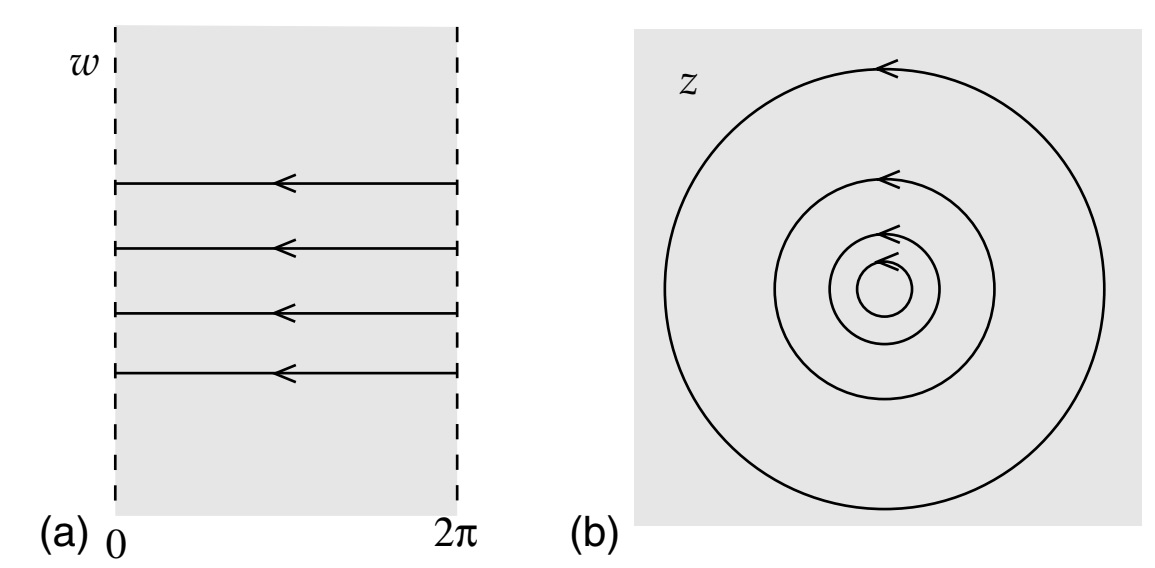
\includegraphics[width=0.8\textwidth,natwidth=866,natheight=426]{Fig2.3.jpg}\\
	\caption{Closed String Coordinates}
\end{center}
\end{figure}

在w坐标中,时间对应于$\sigma^{2}=\operatorname{Im} w$ 的移动. 在z坐标中,时间径向移动,原点是遥远的过去. 这些坐标通过一个共形变换相关. 对于理论的正则解释,w坐标是自然的,但z坐标也相当有用,并且大多数表达式都写在这个参考系中.\\
对于全纯或反全纯算符,我们可以做Laurent展开
\begin{equation}
T_{z z}(z)=\sum_{m=-\infty}^{\infty} \frac{L_{m}}{z^{m+2}}, \quad \tilde{T}_{\bar{z} \bar{z}}(\bar{z})=\sum_{m=-\infty}^{\infty} \frac{\tilde{L}_{m}}{\bar{z}^{m+2}}
\end{equation}
展开系数称为Virasoro生成元. 由围道积分给出
\begin{equation}\label{2.6.6}
L_{m}=\oint_{C} \frac{d z}{2 \pi i z} z^{m+2} T_{z z}(z)
\end{equation}
其中C以逆时针围绕原点的任意围道. 在$\sigma^2=0$时,Laurent展开就是一个普通的Fourier变换
\begin{subequations}
\begin{equation}
T_{w w}(w)=-\sum_{m=-\infty}^{\infty} \exp \left(i m \sigma^{1}-m \sigma^{2}\right) T_{m}
\end{equation}
\begin{equation}
T_{\bar{w} \bar{w}}(\bar{w})=-\sum_{m=-\infty}^{\infty} \exp \left(-i m \sigma^{1}-m \sigma^{2}\right) \tilde{T}_{m}
\end{equation}
\end{subequations}
其中
\begin{equation}\label{2.6.8}
T_{m}=L_{m}-\delta_{m, 0} \frac{c}{24}, \quad \tilde{T}_{m}=\tilde{L}_{m}-\delta_{m, 0} \frac{\tilde{c}}{24}
\end{equation}
$T_0$的额外偏移源于非张量变换(\ref{2.4.26})
\begin{equation}
T_{w w}=\left(\partial_{w} z\right)^{2} T_{z z}+\frac{c}{24}
\end{equation}
在$w=\sigma^{1}+i \sigma^{2}$系中,时间平移的Hamiltonian 是
\begin{equation}\label{2.6.10}
H=\int_{0}^{2 \pi} \frac{d \sigma^{1}}{2 \pi} T_{22}=L_{0}+\tilde{L}_{0}-\frac{c+\tilde{c}}{24}
\end{equation}
注意Laurent展开中的+2. 在Fourier变换中由于T的共形变换被抵消了. 类似地,一个权重h的全纯场的Laurent展开将在指数上包含h. \\
将时间$\operatorname{Im} w=\ln |z|$为常数的圆上的路径积分剪开. Virasoro生成元变成通常意义上的算符. 由于全纯性,积分(\ref*{2.6.6})独立于C,因而特别地,在时间平移下不变. 即它们是守恒荷,与共形不变相联系的荷. \\
一个重要的事实:流的OPE决定了对应荷的代数. 考察一般荷$Q_{i}, i=1,2$,给定为全纯流的围道积分
\begin{equation}
Q_{i}\{C\}=\oint_{C} \frac{d z}{2 \pi i} j_{i}
\end{equation}
考察组合
\begin{equation}\label{2.6.12}
Q_{1}\left\{C_{1}\right\} Q_{2}\left\{C_{2}\right\}-Q_{1}\left\{C_{3}\right\} Q_{2}\left\{C_{2}\right\}
\end{equation}
围道如图(\ref{Fig2.4}a)所示.\\
\begin{figure}
	\begin{center}
		%	\includegraphics[width=0.8\textwidth,bb=0 0 1299 596]{Fig2.3ClosedStringCoordinates.jpg}\\
		%1px=0.75pt
		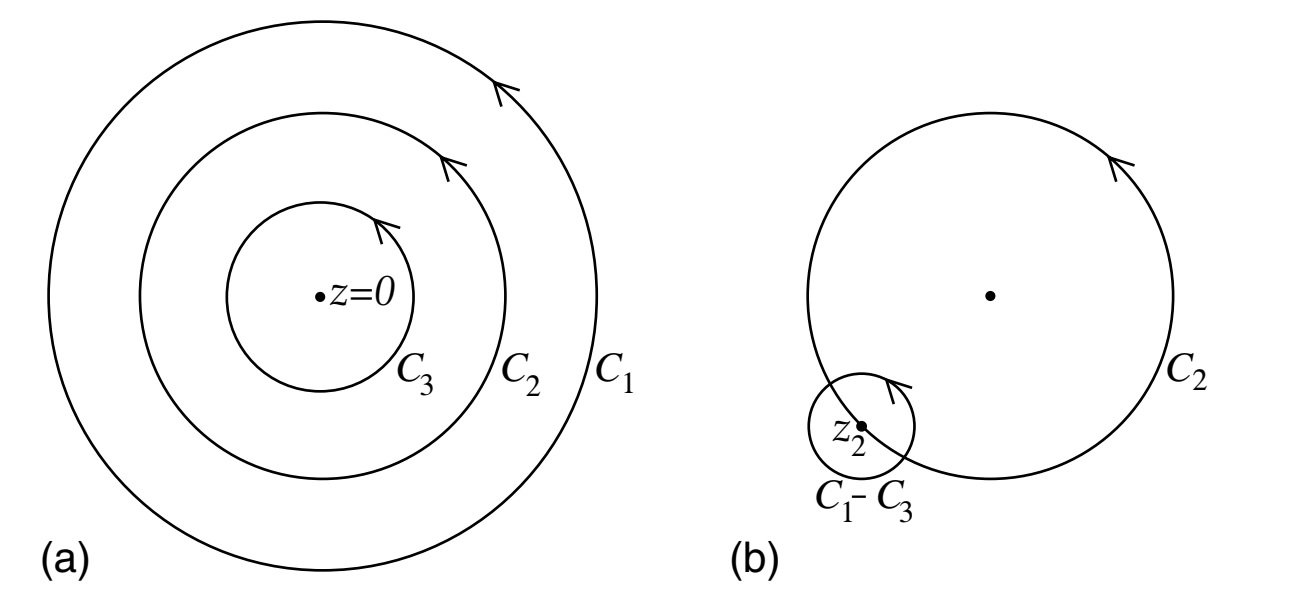
\includegraphics[width=0.8\textwidth,natwidth=974,natheight=447]{Fig2.4.jpg}\\
		\caption{Contours}\label{Fig2.4}
	\end{center}
\end{figure}

因子写成的序列是无关的,因为它们仅是一个路径积分中的积分变量(除非两个荷是反对易的. 在这种情况下会有一个额外的符号并且所有的对易子都会变成反对易子).\\
正如附录中所讨论的,当我们劈开路径积分以做一个算符解释. 决定算符序列的是时间顺序,在这里是
$t_{1}>t_{2}>t_{3}$. 对组合(\ref{2.6.12})的路径积分对应矩阵元
\begin{equation}
\hat{Q}_{1} \hat{Q}_{2}-\hat{Q}_{2} \hat{Q}_{1} \equiv\left[\hat{Q}_{1}, \hat{Q}_{2}\right]
\end{equation}
现在,对于围道$C_2$上的一给定点$z_2$,我们可以将$C_1, C_3$围道的差异进行变形,如图(\ref{Fig2.4}b)所示.\\
对易子因而由OPE的留数给出
\begin{equation}
\left[Q_{1}, Q_{2}\right]\left\{C_{2}\right\}=\oint_{C_{2}} \frac{d z_{2}}{2 \pi i} \operatorname{Res}_{z_{1} \rightarrow z_{2}} j_{1}\left(z_{1}\right) j_{2}\left(z_{2}\right)
\end{equation}
围道讨论允许我们在OPE与对易关系之间来回传递. 我们来强调一下,对于守恒流,知道了OPE中的奇异性等效于知道了对应荷的对易子代数. 将守恒荷$Q_{2}\left\{C_{2}\right\}$ 替换成任意算符,上面的讨论同样适用:
\begin{equation}
\left[Q, \mathscr{A}\left(z_{2}, \bar{z}_{2}\right)\right]=\operatorname{Res}_{z_{1} \rightarrow z_{2}} j\left(z_{1}\right) \mathscr{A}\left(z_{2}, \bar{z}_{2}\right)=\frac{1}{i \epsilon} \delta \mathscr{A}\left(z_{2}, \bar{z}_{2}\right)
\end{equation}
这正是熟悉的陈述:荷Q生成了相对应的变换. 类似地,对于反全纯流的围道积分
\begin{equation}
\tilde{Q}\{C\}=-\oint_{C} \frac{d \bar{z}}{2 \pi i} \tilde{\jmath}
\end{equation}
Ward等式与围道讨论暗示了
\begin{equation}
\left[\tilde{Q}, \mathscr{A}\left(z_{2}, \bar{z}_{2}\right)\right]=\overline{\operatorname{Res}}_{\bar{z}_{1} \rightarrow \bar{z}_{2}} \tilde{\jmath}\left(\bar{z}_{1}\right) \mathscr{A}\left(z_{2}, \bar{z}_{2}\right)=\frac{1}{i \epsilon} \delta \mathscr{A}\left(z_{2}, \bar{z}_{2}\right)
\end{equation}
将其应用于Virasoro代数(\ref{2.6.6}), 
\begin{equation}
\begin{array}{l}
\operatorname{Res}_{z_{1} \rightarrow z_{2}} z_{1}^{m+1} T\left(z_{1}\right) z_{2}^{n+1} T\left(z_{2}\right) \\
\quad=\operatorname{Res}_{z_{1} \rightarrow z_{2}} z_{1}^{m+1} z_{2}^{n+1}\left(\frac{c}{2 z_{12}^{4}}+\frac{2}{z_{12}^{2}} T\left(z_{2}\right)+\frac{1}{z_{12}} \partial T\left(z_{2}\right)\right)\\
=\frac{c}{12}\left(\partial^{3} z_{2}^{m+1}\right) z_{2}^{n+1}+2\left(\partial z_{2}^{m+1}\right) z_{2}^{n+1} T\left(z_{2}\right)+z_{2}^{m+n+2} \partial T\left(z_{2}\right) \\
=\frac{c}{12}\left(m^{3}-m\right) z_{2}^{m+n-1}+(m-n) z_{2}^{m+n+1} T\left(z_{2}\right)+\text { total derivative }
\end{array}
\end{equation}
其中$j_{m}(z)=z^{m+1} T(z)$.
那么右边的$z_2$围道积分给出Virasoro代数:
\begin{equation}\label{2.6.19}
\left[L_{m}, L_{n}\right]=(m-n) L_{m+n}+\frac{c}{12}\left(m^{3}-m\right) \delta_{m,-n}
\end{equation}
$\tilde{L}_{m}$满足中心荷为$\tilde{c}$ 的相同代数.
因而任何CFT有无限个守恒荷,即Virasoro生成元. 其作用在Hilbert空间中并满足代数(\ref{2.6.19}). 先关注几个简单的性质. 一般地,处理$L_{0}$ 和 $\tilde{L}_{0}$ 的本征态,生成元$L_{0}$ 满足
\begin{equation}
\left[L_{0}, L_{n}\right]=-n L_{n}
\end{equation}
如果$|\psi\rangle$ 是 $L_{0}$的本征值为h的本征态,那么
\begin{equation}
L_{0} L_{n}|\psi\rangle=L_{n}\left(L_{0}-n\right)|\psi\rangle=(h-n) L_{n}|\psi\rangle
\end{equation}
所以$L_n|\psi\rangle$ 是本征值为h-n的本征态,n<0的生成元提高$L_{0}$的本征值,而n>0则降低它.\\
三个生成元$L_{0}$ , $L_{\pm 1}$构成没有中心荷的闭代数:
\begin{equation}
\left[L_{0}, L_{1}\right]=-L_{1}, \quad\left[L_{0}, L_{-1}\right]=L_{-1}, \quad\left[L_{1}, L_{-1}\right]=2 L_{0}
\end{equation}
这是代数$SL(2,R)$,与SU(2)相差一个符号. 对于权重$(h,0)$的全纯张量场$\mathcal{O}$的Laurent系数
\begin{equation}
\mathcal{O}(z)=\sum_{m=-\infty}^{\infty} \frac{\mathcal{O}_{m}}{z^{m+h}}
\end{equation}
从OPE(\ref{2.4.16})得到对易子
\begin{equation}
\left[L_{m}, \mathcal{O}_{n}\right]=[(h-1) m-n] \mathcal{O}_{m+n}
\end{equation}
又一次, n>0的模减小$L_0$,n<0的模增大$L_0$.\\
\begin{proof}
令
$j_{m}(z)=z^{m+1} T(z), \quad j_{n}(z)=z^{n+h-1} \mathcal{O}(z)$
$$
\begin{array}{l}
\operatorname{Res}_{z_1 \rightarrow z_2}  z_1^{m+1} T\left(z_{1}\right) z_2^{n+h-1} \mathcal{O}(z_{2})\\
=\operatorname{Res}_{z_1 \rightarrow z_2} z_1^{m+1} z_2^{n+h-1}\left(\frac{h}{z_{12}^2} O(z_2)+\frac{1}{z_{12}} \partial \mathcal{O}(z_2)\right)\\
=h(\partial z_2^{m+1})z_2^{n+h-1}\mathcal{O}(z_2)+z_2^{m+n+h}\partial\mathcal{O}(z_2)\\
=h(m+1)z_2^{m+n+h-1}\mathcal{O}(z_2)-(m+n+h)z_2^{m+n+h-1}\mathcal{O}(z_2)+div
\end{array}
$$
所以第一项
$$h(m+1)z_2^{m+n+h-1}\mathcal{O}(z_2) \sim h(m+1) \sum \mathcal{O}_q z_2^{m+n-q-1} \sim h(m+1)\mathcal{O}_{m+n}$$
第二项
$$
\begin{array}{l}
=-(m+n+h) z_{2}^{m+n+h-1} \sum \frac{\mathcal{O}_{q}}{z_{2}^{q+h}} \\
\sim -(m+n+h) \sum \mathcal{O}_{q} z_{2}^{m+n-q-1} \\
\sim-(m+n+h) \mathcal{O}_{m+n}
\end{array}
$$

二者相加得
$$\left[L_{m}, \mathcal{O}_{n}\right]=[(h-1) m-n] \mathcal{O}_{m+n}$$
\end{proof}

在开弦中,令
\begin{equation}
0 \leq \operatorname{Re} w \leq \pi \quad \Leftrightarrow \quad \operatorname{Im} z \geq 0
\end{equation}
其中
$z=-\exp (-i w)$. 
坐标区域如图(\ref{Fig2.5}).
\begin{figure}
	\begin{center}
		%	\includegraphics[width=0.8\textwidth,bb=0 0 778 341]{Fig2.3ClosedStringCoordinates.jpg}\\
		%1px=0.75pt
		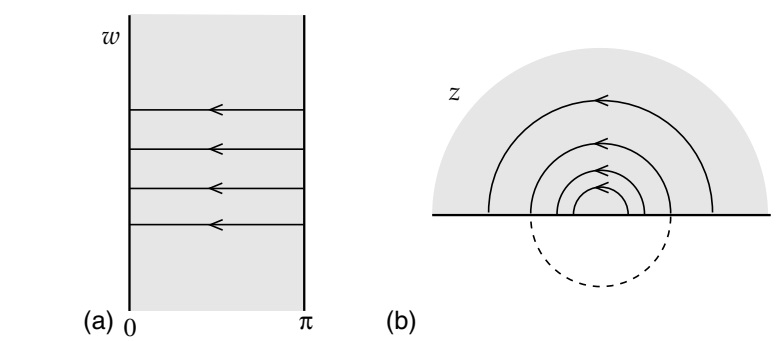
\includegraphics[width=0.8\textwidth,natwidth=584,natheight=256]{Fig2.5.jpg}\\
		\caption{Contours}\label{Fig2.5}
	\end{center}
\end{figure}
作为边界,能动量满足
\begin{equation}\label{2.6.26}
T_{a b} n^{a} t^{b}=0
\end{equation}
其中$n^{a}$ , $t^{b}$是法向和切向矢量. 为了看到这点,考察边界是直线的坐标系. 边界的出现破坏了法向的平移不变性,但不破坏切向,使得流$T_{a b} t^{b}$ 依旧是守恒的. 那么边界条件(\ref{2.6.26})就是陈述流出边界的流是零. 在目前的情况下,这变成
\begin{equation}
T_{w w}=T_{\bar{w} \bar{w}}, \operatorname{Re} w=0, \pi \quad \Leftrightarrow \quad T_{z z}=T_{\bar{z} \bar{z}}, \operatorname{Im} z=0
\end{equation}
使用doubling trick是方便的. 将下半z平面中的$T_{zz}$定义为$T_{\bar{z} \bar{z}}$在上半平面的镜像点$z^{\prime}=\bar{z}$处的值:
\begin{equation}
T_{z z}(z) \equiv T_{\bar{z} \bar{z}}\left(\bar{z}^{\prime}\right), \quad \operatorname{Im} z<0
\end{equation}
运动方程与边界条件总结为:$T_{z z}$在整个复平面全纯.
仅存在一组Virasoro代数,因为边界条件耦合了$T$ 和 $\widetilde{T}$:
\begin{equation}
\begin{aligned}
L_{m} &=\frac{1}{2 \pi i} \int_{C}\left(d z z^{m+1} T_{z z}-d \bar{z} \bar{z}^{m+1} T_{\bar{z} \bar{z}}\right) \\
&=\frac{1}{2 \pi i} \oint d z z^{m+1} T_{z z}(z)
\end{aligned}
\end{equation}
第一行中,围道是中心为原点的半圆;第二行,我们使用了doubling trick将$L_m$写成了闭合围道. 又一次,这些情况满足Virasoro代数
\begin{equation}
\left[L_{m}, L_{n}\right]=(m-n) L_{m+n}+\frac{c}{12}\left(m^{3}-m\right) \delta_{m,-n}
\end{equation}

\section{模式展开}%{2.7 Mode expansions}

\centerline{\Large 自由标量}
在自由场论中,场分解成谐振子,并且频谱与能动量张量可以以模的形式上
给出. 我们从闭弦开始. 在$X^\mu$的理论中, $\partial X$ 和 $\bar{\partial} X$是反全纯的. 所以有类似T的Laurent展开:
\begin{equation}\label{2.7.1}
\partial X^{\mu}(z)=-i\left(\frac{\alpha^{\prime}}{2}\right)^{1 / 2} \sum_{m=-\infty}^{\infty} \frac{\alpha_{m}^{\mu}}{z^{m+1}}, \quad \bar{\partial} X^{\mu}(\bar{z})=-i\left(\frac{\alpha^{\prime}}{2}\right)^{1 / 2} \sum_{m=-\infty}^{\infty} \frac{\tilde{\alpha}_{m}^{\mu}}{\bar{z}^{m+1}}
\end{equation}
等效地,
\begin{subequations}\label{2.7.2}
\begin{equation}
\alpha_{m}^{\mu}=\left(\frac{2}{\alpha^{\prime}}\right)^{1 / 2} \oint \frac{d z}{2 \pi} z^{m} \partial X^{\mu}(z)
\end{equation}
\begin{equation}
\tilde{\alpha}_{m}^{\mu}=-\left(\frac{2}{\alpha^{\prime}}\right)^{1 / 2} \oint \frac{d \bar{z}}{2 \pi} \bar{z}^{m} \bar{\partial} X^{\mu}(\bar{z})
\end{equation}
\end{subequations}
 $X^\mu$的单值性暗示着$\alpha_{0}^{\mu}=\tilde{\alpha}_{0}^{\mu}$ ,更进一步,时空平移的Noether流是$i \partial_{a} X^{\mu} / \alpha^{\prime}$ ,所以时空动量
\begin{equation}\label{2.7.3}
p^{\mu}=\frac{1}{2 \pi i} \oint_{C}\left(d z j^{\mu}-d \bar{z} \tilde{\jmath}^{\mu}\right)=\left(\frac{2}{\alpha^{\prime}}\right)^{1 / 2} \alpha_{0}^{\mu}=\left(\frac{2}{\alpha^{\prime}}\right)^{1 / 2} \tilde{\alpha}_{0}^{\mu}
\end{equation}
对表达式(\ref{2.7.1}) 积分给出
\begin{equation}
X^{\mu}(z, \bar{z})=x^{\mu}-i \frac{\alpha^{\prime}}{2} p^{\mu} \ln |z|^{2}+i\left(\frac{\alpha^{\prime}}{2}\right)^{1 / 2} \sum_{m=-\infty , m \neq 0}^{\infty} \frac{1}{m}\left(\frac{\alpha_{m}^{\mu}}{z^{m}}+\frac{\tilde{\alpha}_{m}^{\mu}}{\bar{z}^{m}}\right)
\end{equation}
无论是从标准正则对易出发,还是从围道讨论或者XXOPE,可以给出
\begin{subequations}
\begin{equation}
\left[\alpha_{m}^{\mu}, \alpha_{n}^{v}\right]=\left[\tilde{\alpha}_{m}^{\mu}, \tilde{\alpha}_{n}^{v}\right]=m \delta_{m,-n} \eta^{\mu v}
\end{equation}
\begin{equation}
\left[x^{\mu}, p^{v}\right]=i \eta^{\mu v}
\end{equation}
\end{subequations}
其他对易子为零. 这个谱通过从态$|0 ; k\rangle$ 开始而给出. 这个态动量为$k^\mu$ 且被所有下降模n>0 的$\alpha_n^\mu$ 所湮灭 而对上升模(n<0) ,则以所有可能的方式作用.\\
我们现在希望以模算符的形式展开Virasoro生成元. 将$X^\mu$ 的Laurent展开式插入到能动量张量(\ref{2.4.4}) 并集合z的给定阶的项,给出
\begin{equation}\label{2.7.6}
L_{m} \sim \frac{1}{2} \sum_{n=-\infty}^{\infty} \alpha_{m-n}^{\mu} \alpha_{\mu n}
\end{equation}
 ~代表我们忽略了算符的顺序. 对于$m\neq 0$ , 展开式(\ref{2.7.6}) 是定义良好的且正确的————每一项的模算符对易所以序列不重要. 对于m=0, 将下降算符放在右边并引入一规范序列常数
 \begin{equation}
 L_{0}=\frac{\alpha^{\prime} p^{2}}{4}+\sum_{n=1}^{\infty}\left(\alpha_{-n}^{\mu} \alpha_{\mu n}\right)+a^{X}
 \end{equation}
 我们在1.3节中遇到同一问题,在那里我们以一种启发式的方法处理 现在左边以::一序列能动量张量的Laurent系数的形式有了一个有限且明确的定义,所以规范序列常数是有限且可计算的. 有几种方式可以决定它,最简单的是用Virasoro代数:
 \begin{equation}\label{2.7.8}
 2 L_{0}|0 ; 0\rangle=\left(L_{1} L_{-1}-L_{-1} L_{1}\right)|0 ; 0\rangle=0
 \end{equation}
 因而
 \begin{equation}
 a^{X}=0
 \end{equation}
 这里我们使用了$L_1, L_{-1}$ 的已知形式:每一项要么包含下降算符,要么包含$p^\mu$. 因而湮灭$|0 ; 0\rangle$. \\
从OPE中,我们决定了Virasoro代数的中心荷. 它也可以从Virasoro代数的模算符表达式直接得出.\\
引入一个新的记法. 符号${}_\circ^\circ {}_\circ^\circ$ 代表产生-湮灭正规序列,将所有下降算符放在所有产生算符右边. 注意交换反对易算符时有一个负号. 由于这个原因,我们将$p^\mu$纳入下降算符,将$x^\mu$纳入上升算符. 在这个记号下,我么可以写
\begin{equation}\label{2.7.10}
L_{m}=\frac{1}{2} \sum_{n=-\infty}^{\infty}{}_{\circ}^{\circ} \alpha_{m-n}^{\mu} \alpha_{\mu n}{}_{\circ}^{\circ}
\end{equation}
我们现在引入了两种正规序列形式,即共形正规序列::与产生-湮灭正规序列${}_\circ^\circ {}_\circ^\circ$ . 前者是有用的,因为它所产生的算符,其OPE与共形变换性质是简单的;后者可能对于读者更为熟悉,在处理算符的矩阵元时是有用的. 我们现在要给出二者关系. 从比较编时乘积与产生-湮灭正规乘积开始. 对于 $|z|>\left|z^{\prime}\right|$的乘积$X^{\mu}(z, \bar{z}) X^{\nu}\left(z^{\prime}, \bar{z}^{\prime}\right)$ ,代入模展开,并将$X^{\mu}(z, \bar{z})$ 中的下降算符挪到右边,保留对易子的痕迹给出
\begin{equation}\label{2.7.11}
\begin{aligned}
X^{\mu}(z, \bar{z}) X^{\nu}\left(z^{\prime}, \bar{z}^{\prime}\right)=&{ }_{\circ}^{\circ} X^{\mu}(z, \bar{z}) X^{\nu}\left(z^{\prime}, \bar{z}^{\prime}\right)  { }_{\circ}^{\circ} \\
&+\frac{\alpha^{\prime}}{2} \eta^{\mu \nu}\left[-\ln |z|^{2}+\sum_{m=1}^{\infty} \frac{1}{m}\left(\frac{z^{\prime m}}{z^{m}}+\frac{\bar{z}^{\prime m}}{\bar{z}^{m}}\right)\right]\\
=&{ }_{\circ}^{\circ} X^{\mu}(z, \bar{z}) X^{\nu}\left(z^{\prime}, \bar{z}^{\prime}\right)  { }_{\circ}^{\circ}-\frac{\alpha^{\prime}}{2} \eta^{\mu \nu}\ln |z-z^\prime|^{2}
\end{aligned}
\end{equation}
由于$|z|>\left|z^{\prime}\right|$,这里左边是编时的而且求和收敛. 定义(2.1.21)给出的编时乘积与共形正规乘积的关系(以路径积分语言,所以右边的乘积在算符体系下是编时的). 这与(\ref{2.7.11})是相同的,使得
\begin{equation}\label{2.7.12}
{ }_\circ^{\circ} X^{\mu}(z, \bar{z}) X^{\nu}\left(z^{\prime}, \bar{z}^{\prime}\right){}_\circ^{\circ}=: X^{\mu}(z, \bar{z}) X^{\nu}\left(z^{\prime}, \bar{z}^{\prime}\right):
\end{equation}
这种关系在普遍的CFT中并不成立,并且实际上,$p^\mu$与下降算符的某些组合给出更简单的结果. 对于算符的w形式的共形正规序列这也不成立.
从(\ref{2.7.12})可以立即写出模展开(\ref{2.7.10}) 给出$a^x=0$的二阶导数.\\
超过两个$X^\mu$的产生-湮灭正规乘积与::序列有相同的组合学因子. 即,它们从编时乘积中,通过对所有的收缩获得(场论中的Wick定理). 为了将算符的正规序列从一种形式转化到另一种形式,利用两点函数的差对所有收缩求和. 即,如果我们有两类序列
\begin{equation}
\left[X^{\mu}(z, \bar{z}) X^{v}\left(z^{\prime}, \bar{z}^{\prime}\right)\right]_{1}=\left[X^{\mu}(z, \bar{z}) X^{v}\left(z^{\prime}, \bar{z}^{\prime}\right)\right]_{2}+\eta^{\mu v} \Delta\left(z, \bar{z}, z^{\prime}, \bar{z}^{\prime}\right)
\end{equation}
那么对于一般算符$\mathscr{F}$
\begin{equation}
[\mathscr{F}]_{1}=\exp \left(\frac{1}{2} \int d^{2} z d^{2} z^{\prime} \Delta\left(z, \bar{z}, z^{\prime}, \bar{z}^{\prime}\right) \frac{\delta}{\delta X^{\mu}(z, \bar{z})} \frac{\delta}{\delta X_{\mu}\left(z^{\prime}, \bar{z}^{\prime}\right)}\right)[\mathscr{F}]_{2}
\end{equation}
对于线性伸缩子CFT,Laurent展开与对易子不变,而Virasoro生成元包含一个额外项
\begin{equation}
L_{m}=\frac{1}{2} \sum_{n=-\infty}^{\infty}{}_{\circ}^{\circ} \alpha_{m-n}^{\mu} \alpha_{\mu n}{}_{\circ}^{\circ}+i\left(\frac{\alpha^{\prime}}{2}\right)^{1 / 2}(m+1) V^{\mu} \alpha_{\mu m}
\end{equation}

\centerline{\Large bc CFT}
场b和c有Laurent展开
\begin{equation}
b(z)=\sum_{m=-\infty}^{\infty} \frac{b_{m}}{z^{m+\lambda}}, \quad c(z)=\sum_{m=-\infty}^{\infty} \frac{c_{m}}{z^{m+1-\lambda}}
\end{equation}
精确些,如果$\lambda$是整数,它们仅是Laurent展开. 半整数的情况也是有趣的,我们将在第10章细致地处理它. OPE给出反对易子
\begin{equation}
\left\{b_{m}, c_{n}\right\}=\delta_{m,-n}
\end{equation}
首先考察被所有n>0的算符消灭的态. $b_0, c_0$振子代数生成两个这样的基态$|\downarrow\rangle$ 和 $|\uparrow\rangle$. 其有性质
\begin{subequations}
\begin{equation}
b_{0}|\downarrow\rangle=0, \quad b_{0}|\uparrow\rangle=|\downarrow\rangle,
\end{equation}
\begin{equation}
c_{0}|\downarrow\rangle=|\uparrow\rangle, \quad c_{0}|\uparrow\rangle=0,
\end{equation}
\begin{equation}
b_{n}|\downarrow\rangle=b_{n}|\uparrow\rangle=c_{n}|\downarrow\rangle=c_{n}|\uparrow\rangle=0, \quad n>0
\end{equation}
\end{subequations}
普通的态通过用n<0的模作用其上获得,不过由于反对易,最多作用一次. 由于之后的某些原因,将$b_0$与下降算符组队,$c_0$与上升算符组队将是方便的,所以我们挑出$|\downarrow\rangle$ 作为幽灵真空$|0\rangle$.在弦论中我们将有一个全纯bc理论,与反全纯$\tilde{b} \tilde{c}$ 理论. 每一个有$\lambda=2$,因而闭弦频谱包含之上的两个的乘积.\\
Virasoro生成元是
\begin{equation}
L_{m}=\sum_{n=-\infty}^{\infty}(m \lambda-n) {}_\circ^\circ b_{n} c_{m-n}{}_\circ^\circ+\delta_{m, 0} a^{\mathrm{g}}
\end{equation}
序列常数. 可以(\ref{2.7.8})那样决定,其给出
\begin{equation}
\begin{aligned}
2 L_{0}|\downarrow\rangle &=\left(L_{1} L_{-1}-L_{-1} L_{1}\right)|\downarrow\rangle \\
&=\left(\lambda b_{0} c_{1}\right)\left[(1-\lambda) b_{-1} c_{0}\right]|\downarrow\rangle=\lambda(1-\lambda)|\downarrow\rangle
\end{aligned}
\end{equation}
因而$a^{\mathrm{g}}=\frac{1}{2} \lambda(1-\lambda)$
并且
\begin{equation}
L_{m}=\sum_{n=-\infty}^{\infty}(m \lambda-n) {}_\circ^\circ b_{n} c_{m-n}{}_\circ^\circ+\frac{\lambda(1-\lambda)}{2} \delta_{m, 0}
\end{equation}
常数也可以通过解出::和${}_\circ^\circ {}_\circ^\circ$的关系获得. 对于幽灵数流(\ref{2.5.14}),  荷是
\begin{equation}\label{2.7.22}
\begin{aligned}
N^{\mathrm{g}} &=-\frac{1}{2 \pi i} \int_{0}^{2 \pi} d w j_{w} \\
&=\sum_{n=1}^{\infty}\left(c_{-n} b_{n}-b_{-n} c_{n}\right)+c_{0} b_{0}-\frac{1}{2}
\end{aligned}
\end{equation}
它满足
\begin{equation}
\left[N^{\mathrm{g}}, b_{m}\right]=-b_{m}, \quad\left[N^{\mathrm{g}}, c_{m}\right]=c_{m}
\end{equation}
因而c数减去b数是激发. 基态有鬼数$\pm \frac{1}{2}$
\begin{equation}
N^{\mathrm{g}}|\downarrow\rangle=-\frac{1}{2}|\downarrow\rangle, \quad N^{\mathrm{g}}|\uparrow\rangle=\frac{1}{2}|\uparrow\rangle
\end{equation}
这依赖于序列常数的值,可以进行猜测. 理由是基态平均幽灵数应该是零:鬼数在$b \leftrightarrow c$ 下改变符号.\\

\centerline{\Large 开弦}
在开弦中,Neumann边界条件变成了实轴上的$\partial_z X^{\mu}=\partial_{\bar{z}} X^{\mu}$.
仅存在一组模,边界条件要求展开式(\ref{2.7.1})中$\alpha_{m}^{\mu}=\tilde{\alpha}_{m}^{\mu}$. 时空动量积分 (\ref{2.7.3})只积半圆. 所以现在的归一化是
\begin{equation}
\alpha_{0}^{\mu}=\left(2 \alpha^{\prime}\right)^{1 / 2} p^{\mu}
\end{equation}
那么$X^\mu$的展开是
\begin{equation}
X^{\mu}(z, \bar{z})=x^{\mu}-i \alpha^{\prime} p^{\mu} \ln |z|^{2}+i\left(\frac{\alpha^{\prime}}{2}\right)^{1 / 2} \sum_{m=-\infty , m \neq 0}^{\infty} \frac{\alpha_{m}^{\mu}}{m}\left(z^{-m}+\bar{z}^{-m}\right)
\end{equation}
另外
\begin{equation}
L_{0}=\alpha^{\prime} p^{2}+\sum_{n=1}^{\infty} \alpha_{-n}^{\mu} \alpha_{\mu n}
\end{equation}
对易子像往常一样
\begin{equation}
\left[\alpha_{m}^{\mu}, \alpha_{n}^{\nu}\right]=m \delta_{m,-n} \eta^{\mu \nu}, \quad\left[x^{\mu}, p^{\nu}\right]=i \eta^{\mu \nu}
\end{equation}
对于bc理论,与弦相关的边界条件是
\begin{equation}
c(z)=\tilde{c}(\bar{z}), \quad b(z)=\tilde{b}(\bar{z}), \quad \operatorname{Im} z=0
\end{equation}
这是z坐标形式,其中边界在实轴上. 那么我们可以用双倍叠加将上半平面的全纯场和反全纯场写成整个平面中的全纯场的形式
\begin{equation}
c(z) \equiv \tilde{c}\left(\bar{z}^{\prime}\right), \quad b(z) \equiv \tilde{b}\left(\bar{z}^{\prime}\right), \quad \operatorname{Im}(z) \leq 0, z^{\prime}=\bar{z}
\end{equation}
因而对于单个b和c,开弦有单组Laurent展开.

\section{顶角算子}%{2.8 Vertex operators}

在量子场论中,一方面,既有理论的态空间;另一方面,又有定域算符的集合. 在共形场论中,它们之间有一个简单且有用的同构,CFT在一个圆上量子化. 考察w坐标中半无限大的圆柱
\begin{equation}
0 \leq \operatorname{Re} w \leq 2 \pi, \quad w \sim w+2 \pi, \quad \operatorname{Im} w \leq 0
\end{equation}
其映射到$z=\exp (-i w)$ 下的一个单位圆盘.  如图(\ref{Fig2.6})所示.
\begin{figure}
\begin{center}
		%	\includegraphics[width=0.8\textwidth,bb=0 0 714 503]{Fig2.3ClosedStringCoordinates.jpg}\\
		%1px=0.75pt
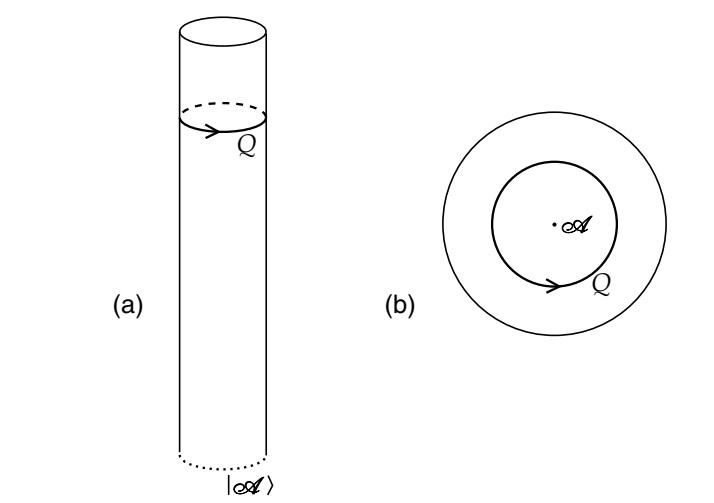
\includegraphics[width=0.8\textwidth,natwidth=535,natheight=377]{Fig2.6.jpg}\\
\caption{(a) A semi-infinite cylinder in w, with initial state $|\mathscr{A}\rangle$ and charge Q. 
(b)The conformally equivalent unit disk with local operator $\mathscr{A}$ and contour integral for Q}\label{Fig2.6}
\end{center}
\end{figure}
对于自由场论,容易得到这个同构的详细形式. 假定有一守恒荷Q以图(\ref{Fig2.6}a)那样的方式作用在态$|\mathscr{A}\rangle$ 上. 通过使用OPE计算图(\ref{Fig2.6}b)中的围道积分,可以发现对应的定域算符. 对应于单位算符,我们等同态$|1\rangle$. 在原点没有算符时,$\partial X^{\mu}$ 和 $\bar{\partial} X^{\mu}$在图(\ref{Fig2.6}b)Q的围道内是全纯和反全纯的. 那么,定义$m \geq 0$ 的$\alpha_{m}^{\mu}$ and $\tilde{\alpha}_{m}^{\mu}$的围道积分(\ref{2.7.2})没有极点因而为零. 因而$|1\rangle$ 被这些模消灭,这表明它是基态
\begin{equation}
|1\rangle=|0 ; 0\rangle
\end{equation}
现在考察,例如m为正的态$\alpha_{-m}^{\mu}|1\rangle$. 过渡到图(\ref{Fig2.6}b),$Q=\alpha_{-m}^{\mu}$,场在围道内是全纯的
\begin{equation}\label{2.8.3}
\alpha_{-m}^{\mu}=\left(\frac{2}{\alpha^{\prime}}\right)^{1 / 2} \oint \frac{d z}{2 \pi} z^{-m} \partial X^{\mu}(z) \rightarrow\left(\frac{2}{\alpha^{\prime}}\right)^{1 / 2} \frac{i}{(m-1) !} \partial^{m} X^{\mu}(0)
\end{equation}
因而
\begin{equation}
\alpha_{-m}^{\mu}|1\rangle \cong\left(\frac{2}{\alpha^{\prime}}\right)^{1 / 2} \frac{i}{(m-1) !} \partial^{m} X^{\mu}(0), \quad m \geq 1
\end{equation}
类似地
\begin{equation}
\tilde{\alpha}_{-m}^{\mu}|1\rangle \cong\left(\frac{2}{\alpha^{\prime}}\right)^{1 / 2} \frac{i}{(m-1) !} \bar{\partial}^{m} X^{\mu}(0), \quad m \geq 1
\end{equation}
当$\alpha_{-m}^{\mu}$ or $\tilde{\alpha}_{-m}^{\mu}$ 作用在一般态$|\mathscr{A}\rangle$上时,这个对应依旧成立. 如果$: \mathscr{A}(0,0):$ 是任意的正规序列算符,在$\partial X^{\mu}(z)$ 与 $: \mathscr{A}(0,0)$ : 的算符乘积中可能会有奇异性. 但不难验证
\begin{equation}
\alpha_{-m}^{\mu}: \mathscr{A}(0,0):=: \alpha_{-m}^{\mu} \mathscr{A}(0,0):
\end{equation}
对于m>0成立. 这是因为该收缩的围道积分将不可能有单奇点,那么可以在正规序列中进行相同的运算(\ref{2.8.3}). 因而有数个$\alpha$振子激发的态作为相对应算符的::正规乘积出现
\begin{subequations}\label{2.8.7}
\begin{equation}
\alpha_{-m}^{\mu} \rightarrow i\left(\frac{2}{\alpha^{\prime}}\right)^{1 / 2} \frac{1}{(m-1) !} \partial^{m} X^{\mu}(0), \quad m \geq 1
\end{equation}
\begin{equation}
\tilde{\alpha}_{-m}^{\mu} \rightarrow i\left(\frac{2}{\alpha^{\prime}}\right)^{1 / 2} \frac{1}{(m-1) !} \bar{\partial}^{m} X^{\mu}(0), \quad m \geq 1
\end{equation}
\end{subequations}
类似地
\begin{equation}\label{2.8.8}
x_{0}^{\mu} \rightarrow X^{\mu}(0,0)
\end{equation}
通过用(\ref{2.8.7}) 和(\ref{2.8.8}) 左边的算符作用在$|1\rangle$ 上可以获得任何算符. 那么对应该态的算符由右边相对应的定域算符的::正规乘积给定. 例如
\begin{equation}
|0 ; k\rangle \cong: e^{i k \cdot X(0,0)}:
\end{equation}
这是很容易理解的:在平移$X^{\mu} \rightarrow X^{\mu}+a^{\mu}$ 下,态与相对应算符由同一平移, 被乘以$\me ^{\mi ka}$. \\
同一方法适用于bc理论. 明晰起见,我们指定$\lambda=2$的情况. 这是Boson弦论感兴趣的. 从Laurent展开与围道讨论给出
\begin{equation}\label{2.8.10}
b_{m}|1\rangle=0, \quad m \geq-1, \quad c_{m}|1\rangle=0, \quad m \geq 2
\end{equation}
注意Laurent展开指数中的飘移,它源于b和c的共形权重. 单位算符不再映射到基态上. 反而,关系(\ref{2.8.10})决定了
\begin{equation}
|1\rangle=b_{-1}|\downarrow\rangle
\end{equation}
上升算符的平移是直接的
\begin{subequations}
\begin{equation}
b_{-m} \rightarrow \frac{1}{(m-2) !} \partial^{m-2} b(0), \quad m \geq 2
\end{equation}
\begin{equation}
c_{-m} \rightarrow \frac{1}{(m+1) !} \partial^{m+1} c(0), \quad m \geq-1
\end{equation}
\end{subequations}
注意,鬼数为-3/2的态$b_{-1}|\downarrow\rangle$映射到鬼数为0的单位算符,而鬼数为-1/2的态$|\downarrow\rangle$映射到鬼数为1的算符c. 这一差异源于鬼数流的非张量性质(\ref{2.5.17})
\begin{equation}
\left(\partial_{z} w\right) j_{w}(w)=j_{z}(z)+q_{0} \frac{\partial_{z}^{2} w}{\partial_{z} w}=j_{z}(z)-\frac{q_{0}}{z}
\end{equation}
其中$q_{0}=\lambda-\frac{1}{2}=\frac{3}{2}$. 圆柱参考系表达式(\ref{2.7.22})通常定义了态的鬼数,而图(\ref{Fig2.6})的围道讨论将顶点算符的鬼数与极坐标系荷关系起来
\begin{equation}
Q^{\mathrm{g}} \equiv \frac{1}{2 \pi i} \oint d z j_{z}=N^{\mathrm{g}}+q_{0}
\end{equation}
这也适用于其他荷:对于张量流,态与相对应算符的荷是相等的.\\
上面大多数讨论可扩张到$\beta\gamma$理论,但在超弦下存在一定困难. \\
本节所有概念可扩展至开弦,半无限大带
\begin{equation}
0 \leq \operatorname{Re} w \leq \pi, \quad \operatorname{Im} w \leq 0
\end{equation}
映射至一个半圆盘;上半平面与单位圆的交叠映射为$z=-\exp (-i w)$;初态又一次映射至原点,其在边界上,所以存在同构
\begin{equation}
\text { local operators on the boundary边界上的局域算符 } \leftrightarrow \text { states on the interval 交界上的态}
\end{equation}
细节与之上相同. 双重技巧在围道讨论中是有用的.

\centerline{\Large 路径积分推导}
考察z平面的一个圆盘,其在原点处有定域算符$\mathscr{A}$,并在路径积分场中,在单位圆上取固定的边界值$\phi_{\mathrm{b}}$,对圆盘内部场$\phi_i$的路径积分且$\phi_{\mathrm{b}}$保持固定产生了泛函$\Psi_{\mathscr{A}}[\phi_{\mathrm{b}}]$
\begin{equation}
	\Psi_{\mathscr{A}}\left[\phi_{\mathrm{b}}\right]=\int\left[d \phi_{\mathrm{i}}\right]_{\phi_{\mathrm{b}}} \exp \left(-S\left[\phi_{\mathrm{i}}\right]\right) \mathscr{A}(0)
\end{equation}
场的泛函是态的Schrodinger表示,所以这是从算符到态的映射Schrodinger表示,其为每个场构形赋予了一个复振幅,有很多用途.\\
以另一种方式,从某个态$\Psi[\phi_{\mathrm{b}}]$开始. 考察在圆环区域$1 \geq|z| \geq r$ 上的路径积分,其中外圆上的$\phi_{\mathrm{b}}$ 固定,而沿着内圆对$\phi_{\mathrm{b}}^\prime$ 作如下积分:
\begin{equation}\label{2.8.18}
\int\left[d \phi_{\mathrm{b}}^{\prime}\right]\left[d \phi_{\mathrm{i}}\right]_{\phi_{\mathrm{b}}, \phi_{\mathrm{b}}^{\prime}} \exp \left(-S\left[\phi_{\mathrm{i}}\right]\right) r^{-L_{0}-\tilde{L}_{0}} \Psi\left[\phi_{\mathrm{b}}^{\prime}\right]
\end{equation}
即这个积分被赋予权重$r^{-L_{0}-\tilde{L}_{0}} \Psi\left[\phi_{\mathrm{b}}^{\prime}\right]$. 现在,对圆盘的路径积分恰好对应从 $|z|=r$到 $|z|=1$的传播,其等价于用算符 $r^{+L_{0}+\tilde{L}_{0}}$作用. 这抵消了作用在$\Phi$上的算符,所以(\ref{2.8.18})又一次是
$\Psi[\phi_{\mathrm{b}}]$. 现在取$r\to 0$的极限,圆环变成圆盘,而在内圆上的路径积分极限可以认为是在原点处定义了某个定域算符. 通过构建,圆盘上的路径积分与这个算符重新产生了边界上的$\Psi[\phi_{\mathrm{b}}]$. 我们来显示地处理单自由标量场X. 在单位圆上展开
\begin{equation}
X_{\mathrm{b}}(\theta)=\sum_{n=-\infty}^{\infty} X_{n} e^{i n \theta}, \quad X_{n}^{*}=X_{-n}
\end{equation}
边界态$\Psi[X_b]$可以认为是所有$X_n$的函数. 首先辨认出对应于单位算符的态. 由无插入的路径积分给定
\begin{equation}
\Psi_{1}\left[X_{\mathrm{b}}\right]=\int\left[d X_{\mathrm{i}}\right]_{X_{\mathrm{b}}} \exp \left(-\frac{1}{2 \pi \alpha^{\prime}} \int d^{2} z \partial X \bar{\partial} X\right)
\end{equation}
通过通常的Gauss法计算它. 将$X_i$分解成经典部分与涨落
\begin{subequations}
\begin{equation}
X_{\mathrm{i}}=X_{\mathrm{cl}}+X_{\mathrm{i}}^{\prime}
\end{equation}
\begin{equation}
X_{\mathrm{cl}}(z, \bar{z})=X_{0}+\sum_{n=1}^{\infty}\left(z^{n} X_{n}+\bar{z}^{n} X_{-n}\right)
\end{equation}
\end{subequations}
在这个定义下,$X_{cl}$满足运动方程. $X_i^\prime$在边界上为零. 那么路径积分分成
\begin{equation}
\Psi_{1}\left[X_{\mathrm{b}}\right]=\exp \left(-S_{\mathrm{cl}}\right) \int\left[d X_{\mathrm{i}}^{\prime}\right]_{X_{\mathrm{b}}=0} \exp \left(-\frac{1}{2 \pi \alpha^{\prime}} \int d^{2} z \partial X^{\prime} \bar{\partial} X^{\prime}\right)
\end{equation}
其中
\begin{equation}
\begin{aligned}
S_{\mathrm{cl}} &=\frac{1}{2 \pi \alpha^{\prime}} \sum_{m, n=1}^{\infty} m n X_{m} X_{-n} \int_{|z|<1} d^{2} z z^{m-1} \bar{z}^{n-1} \\
&=\frac{1}{\alpha^{\prime}} \sum_{m=1}^{\infty} m X_{m} X_{-m}
\end{aligned}
\end{equation}
$X_i^\prime$积分是常数,独立于边界条件
\begin{equation}\label{2.8.24}
\Psi_{1}\left[X_{\mathrm{b}}\right] \propto \exp \left(-\frac{1}{\alpha^{\prime}} \sum_{m=1}^{\infty} m X_{m} X_{-m}\right)
\end{equation}
这是Gauss型. 实际上是基态. 为了看到这点,在Schrodinger基下写出上升下降算符
\begin{subequations}
\begin{equation}
\alpha_{n}=-\frac{i n}{\left(2 \alpha^{\prime}\right)^{1 / 2}} X_{-n}-i\left(\frac{\alpha^{\prime}}{2}\right)^{1 / 2} \frac{\partial}{\partial X_{n}}
\end{equation}
\begin{equation}
\tilde{\alpha}_{n}=-\frac{i n}{\left(2 \alpha^{\prime}\right)^{1 / 2}} X_{n}-i\left(\frac{\alpha^{\prime}}{2}\right)^{1 / 2} \frac{\partial}{\partial X_{-n}}
\end{equation}
\end{subequations}
这来自在$|z|=1$处的Laurent展开以及模代数. 作用于(\ref{2.8.24}),我们发现
\begin{equation}
\alpha_{n} \Psi_{1}\left[X_{\mathrm{b}}\right]=\tilde{\alpha}_{n} \Psi_{1}\left[X_{\mathrm{b}}\right]=0, \quad n \geq 0
\end{equation}
所以这确实是基态,因而
\begin{equation}
|1\rangle \propto|0 ; 0\rangle
\end{equation}
不是试用保持路径积分在该点上的总归一化因子,我们定义$|1\rangle =|0 ; 0\rangle$.\\
另一简单计算是对应$\partial^{k} X$ 的态;这仅是给结果上加了一个因子$\partial^{k} X_{\mathrm{cl}}(0)=k ! X_{k}$. 所以
\begin{equation}
\left|\partial^{k} X\right\rangle=k ! X_{k} \Psi_{1}=-i\left(\frac{\alpha^{\prime}}{2}\right)^{1 / 2}(k-1) ! \alpha_{-k}|0 ; 0\rangle
\end{equation}
对于$\bar{\partial}^{k} X$ 是类似的. 这扩展到X的导数与指数的所有乘积. 共形正规序列仅抵消了$X_i^\prime$ 路径积分的效应.

\section{关于态和算符的更多介绍}%{2.9 More on states and operators}

\centerline{\Large OPE}
本节我们做一些态-算符对应的其他应用. 第一个是OPE的普遍推广,如图(\ref{Fig2.7})所示.
\begin{figure}
	\begin{center}
		%	\includegraphics[width=0.8\textwidth,bb=0 0 596 515]{Fig2.3ClosedStringCoordinates.jpg}\\
		%1px=0.75pt
		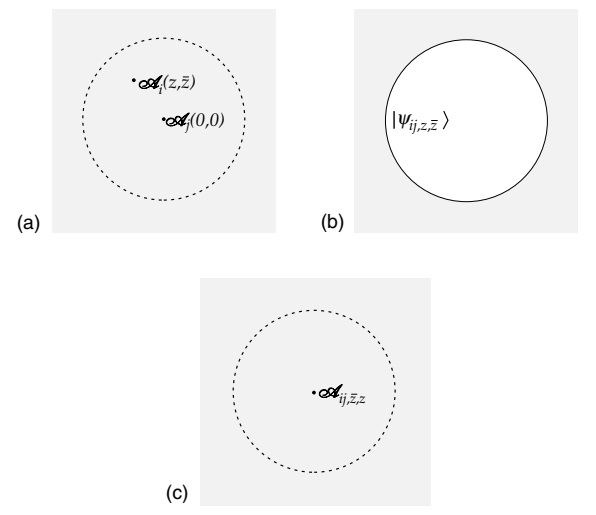
\includegraphics[width=0.8\textwidth,natwidth=370,natheight=300]{Fig2.7.jpg}\\
\caption{(a) World-sheet with two local operators. (b) Integration over fields on the interior of the disk produces boundary state $\left|\psi_{i j, z, \bar{z}}\right\rangle$. (c) Sewing in a disk with the corresponding local operator. Expanding in operators of definite weight gives the OPE.}\label{Fig2.7}
	\end{center}
\end{figure}
考察乘积
\begin{equation}
\mathscr{A}_{i}(z, \bar{z}) \mathscr{A}_{j}(0,0)
\end{equation}
其中$|z|<1$. 我么可以将路径积分分成对单位圆内部场$\phi_i$的积分, 对单位圆上场$\phi_b$的积分,对单位圆外部场$\phi_e$的积分. 正如上节末尾所讨论的,对$\phi_i$的积分给出$\phi_b$的某个泛函,称其为$\Psi_{i j, z, \bar{z}}\left[\phi_{\mathrm{b}}\right]$. 通过态-算符对应,这等价于将圆盘与合适的算符$\mathscr{A}$ 粘在一起. 为了将其变成以$L_{0}, \tilde{L}_{0}$本征态完备集做展开的标准形式
\begin{equation}
\mathscr{A}_{i j, z, \bar{z}}=\sum_{k} z^{h_{k}-h_{i}-h_{j}}-\tilde{h}_{k}-\tilde{h}_{i}-\tilde{h}_{j} c_{i j}^{k} \mathscr{A}_{k}
\end{equation}
其中z相关性与$\bar{z}$相关性像(\ref{2.4.20})中那样由共形权重决定. OPE的收敛性正是量子力学中一个完备集的收敛性. 只要在$\left|z^{\prime}\right| \leq|z|$中没有其他算符,这个构建就是可能的. 使得我们可以剪出半径$|z|+\epsilon$ 的圆.\\
对于三个算符
\begin{equation}
\mathscr{A}_{i}(0,0) \mathscr{A}_{j}(1,1) \mathscr{A}_{k}(z, \bar{z})
\end{equation}
$z\to 0$收敛区域$|z|<1$与$z\to 1$收敛区域$|1-z|<1$重叠. 那么三重积中$\mathscr{A}_l$ 的系数可以写成包含$c_{i k}^{l} c^{m} _{l j}$ 的求和或包含$c_{j k}^{l} c^{m} _{li}$ 的求和. 结合性要求这些和相等. 图解表示见(\ref{Fig2.8}).
\begin{figure}
	\begin{center}
		%	\includegraphics[width=0.8\textwidth,bb=0 0 490 192]{Fig2.3ClosedStringCoordinates.jpg}\\
		%1px=0.75pt
		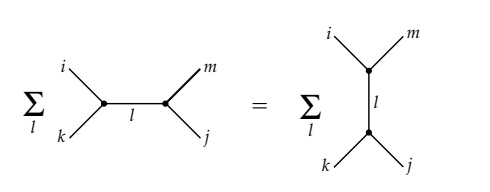
\includegraphics[width=0.8\textwidth,natwidth=300,natheight=110]{Fig2.8.jpg}\\
		\caption{Schematic picture of OPE associativity}\label{Fig2.8}
	\end{center}
\end{figure}
\centerline{\Large Virasoro代数和最高权重态}
现在对Virasoro生成元考察图(\ref{Fig2.6})的讨论:
\begin{equation}
\begin{aligned}
L_{m}|\mathscr{A}\rangle & \cong \oint \frac{d z}{2 \pi i} z^{m+1} T(z) \mathscr{A}(0,0) \\
& \cong L_{m} \cdot \mathscr{A}(0,0)
\end{aligned}
\end{equation}
这里我们进入了新的记法与概念. 给定态-算符同构,作用在Hilbert空间上的每一算符有一个作用在定域算符空间上的像. 换句话说,构成了围绕算符的相应围道并利用OPE计算出所导致的定域算符. 对应将态映射到态的$L_m$是将定域算符映射到定域算符的$L_m$. 一般而言,在不同位置$z_i$处会有定域算符. 对于每一个位置将有一个Virasoro代数的不同版本. 这些不同版本是以算符位置为中心的Laurent展开获得的. 在某些几何中也会存在生成元的一个标准基. 例如对于圆柱以z=0为中心的展开. “·”充当一个提醒:我们所讨论的是围绕特定算符的Laurent展开. \\
在这个记法下,$T\mathscr{A}$OPE是
\begin{equation}\label{2.9.5}
T(z) \mathscr{A}(0,0)=\sum_{m=-\infty}^{\infty} z^{-m-2} L_{m} \cdot \mathscr{A}(0,0)
\end{equation}
为了关联到早期记号(\ref{2.4.11})上,对于$n \geq 0$,$\mathscr{A}^{(n)}=L_{n-1} \cdot \mathscr{A}$ 以及$\mathscr{A}$的共形变换
\begin{equation}
\delta \mathscr{A}(z, \bar{z})=-\epsilon \sum_{n=0}^{\infty} \frac{1}{n !}\left[\partial^{n} v(z) L_{n-1}+\left(\partial^{n} v(z)\right)^{*} \tilde{L}_{n-1}\right] \cdot \mathscr{A}(z, \bar{z})
\end{equation}
利用$T\mathscr{A}$OPE的普遍形式(\ref{2.4.14}),我们有非常有用的结果
\begin{subequations}\label{2.9.7}
\begin{equation}
L_{-1} \cdot \mathscr{A}=\partial \mathscr{A}, \quad \tilde{L}_{-1} \cdot \mathscr{A}=\bar{\partial} \mathscr{A}
\end{equation}
\begin{equation}
L_{0} \cdot \mathscr{A}=h \mathscr{A}, \quad \tilde{L}_{0} \cdot \mathscr{A}=\tilde{h} \mathscr{A}
\end{equation}
\end{subequations}
OPE(\ref{2.9.5})暗示了权重为 $(h, \tilde{h})$的基本场$\mathcal{O}$. 其对应的态满足
\begin{subequations}
\begin{equation}
L_{0}|\mathcal{O}\rangle=h|\mathcal{O}\rangle, \quad \tilde{L}_{0}|\mathcal{O}\rangle=\tilde{h}|\mathcal{O}\rangle
\end{equation}
\begin{equation}
L_{m}|\mathcal{O}\rangle=\tilde{L}_{m}|\mathcal{O}\rangle=0, \quad m>0
\end{equation}
\end{subequations}
这样的态被称为最高权重态. 通过在任意态上重复作用下降算符,我们得到一个态,这个态被进一步的下降算符湮灭,称为最高权重态. \\
一个有趣的特殊情况是单位算符,算符乘积$T1$是非奇异的,所以在任意CFT中得到
\begin{equation}
L_{m}|1\rangle=\tilde{L}_{m}|1\rangle=0, \quad m \geq-1
\end{equation}
正如2.4节所标记的,算符$L_{0}$ 和 $L_{\pm 1}$构成闭代数,$\tilde{L}_{0}$ 和 $\tilde{L}_{\pm 1}$也如此. 全代数是
\begin{equation}
S L(2, \mathbf{C})
\end{equation}
因此$|1\rangle$也称为 $\operatorname{SL}(2, \mathbf{C})$-不变态. 它是唯一一个这样的态. 这是因为(\ref{2.9.7})暗示了对应任何 $\operatorname{SL}(2, \mathbf{C})$-不变态的算符$\mathscr{A}$独立于位置. 那么它必须是c数,正如(\ref{2.4.24}) 之后所解释的. 

\centerline{\Large 幺正CFT}
最高权重态在弦论以及Virasoro代数的表示论中扮演了重要的角色. 现在我们要导出几个在幺正CFT中成立的重要且普遍结果. 幺正CFT有正定内积,这使得
\begin{equation}
L_{m}^{\dagger}=L_{-m}, \quad \tilde{L}_{m}^{\dagger}=\tilde{L}_{-m}
\end{equation}
回忆:内积经由$\langle\alpha \mid A \beta\rangle=\left\langle A^{\dagger} \alpha \mid \beta\right\rangle$ 定义了伴随(adjoint) . 例如$X^\mu$CFT对于类空的$\mu$是幺正的. 如果我们对于基态取内积
\begin{equation}
\left\langle 0 ; k \mid 0 ; k^{\prime}\right\rangle=2 \pi \delta\left(k-k^{\prime}\right)
\end{equation}
并定义
\begin{equation}
\alpha_{m}^{\dagger}=\alpha_{-m}, \quad \tilde{\alpha}_{m}^{\dagger}=\tilde{\alpha}_{-m}
\end{equation}
这隐含地定义了所有更高态的内积. 这个CFT对于$X^\mu=0$不是幺正的,这是因为那里的对易关系存在一个负号. \\
第一个约束是幺正CFT中的任何态都必须有$h, \tilde{h} \geq 0$. 如果这对于最高权重态成立,那么对所有态成立. 对于最高权重态,Virasoro代数给出
\begin{equation}\label{2.9.14}
2 h_{\mathcal{O}}\langle\mathcal{O} \mid \mathcal{O}\rangle=2\left\langle\mathcal{O}\left|L_{0}\right| \mathcal{O}\right\rangle=\left\langle\mathcal{O}\left|\left[L_{1}, L_{-1}\right]\right| \mathcal{O}\right\rangle=\| L_{-1}|\mathcal{O}\rangle \|^{2} \geq 0
\end{equation}
所以$h_{\mathcal{O}} \geq 0 $. 如果 $h_{\mathcal{O}}=\tilde{h}_{\mathcal{O}}=0$,那么得出
\begin{equation}
L_{-1} \cdot \mathcal{O}=\tilde{L}_{-1} \cdot \mathcal{O}=0
\end{equation}
因而 $\mathcal{O}$是独立于位置的. 正如之前所标注的, $\mathcal{O}$必须是c数,即在幺正CFT中单位算符是唯一(0,0)算符. 惊奇的是,$X^\mu$是唯一的例外:相对应的态$x^{\mu}|0 ; 0\rangle$ 由于 $X^\mu$的无限范围是不归一的,并且方程(\ref{2.9.14}) 不再成立. 对于对应紧致维的CFT,一般定理是最有用的,这类例外不可能发生.\\
以同样的方式,在幺正CFT中,当且仅当$\tilde{h}=0$算符是全纯的,当且仅当h=0算符是反全纯的. 这是一个重要结果,我们重复如下:
\begin{equation}
\partial \mathscr{A}=0 \Leftrightarrow h=0, \quad \bar{\partial} \mathscr{A}=0 \Leftrightarrow \tilde{h}=0
\end{equation}
最后,利用之上讨论以及对易子$\left[L_{n}, L_{-n}\right]$,可以证明在幺正CFT中$c, \tilde{c} \geq 0$. 实际上,c=0的唯一幺正CFT是平庸的$L_n$. 

\centerline{\Large 零点能}
态-算符映射给出了另一种不同正规序列常数的简单推导. 在任何CFT中,我们知道$L_{0}|1\rangle=0$ 这决定了$L_0$ 的又一归一化.
在$X$CFT中,$|1\rangle=0$是基态,所以$a^x=0$. 在bc理论中,$|1\rangle=0$是激发态$b_{-1}|\downarrow\rangle$,所以为了与早期$\lambda=2$的结果(\ref{2.7.1}) 一致, $|\downarrow\rangle$的权重是-1.\\
这也提供了中心荷的物理解释. 在幺正CFT中,基态是$L_{0}=\tilde{L}_{0}=0$的$|1\rangle$. 径向生成元与时间平移生成元之间的共形变换(\ref{2.6.10})暗示了. 对于基态
\begin{equation}
E=-\frac{c+\tilde{c}}{24}
\end{equation}
这是Casimir能量,源于系统的有限尺度,且依赖于中心荷. 在量纲背景下,这个能量反比于系统的尺寸$l$,在这里是$2\pi$. 所以一般结果是
\begin{equation}
E=-\frac{\pi(c+\tilde{c})}{12 \ell}
\end{equation}
我们现在有三种计算正规序列常数的方式:
\begin{enumerate}
	\item 像(\ref{2.7.8})中那样,从Virasoro代数出发;
	\item 通过像(\ref{2.7.11})中那样,将正规序列的两种形式关联起来;
	\item 从之上的态-算符映射出发.
\end{enumerate}
然而把零点能加起来的方法是直观的,所以我们给出一种描述,且可以被更加忠实的方法检验:\\
1.对于每个Boson模,零点能为$\frac{1}{2} \omega$;对于每个Fermion模,零点能为$-\frac{1}{2} \omega$. 将能量加起来.\\
2.遇见形式为$\sum_{n=1}^{\infty}(n-\theta)$的发散和, $\theta$  源于非平庸的周期条件,定义其为
\begin{equation}
\sum_{n=1}^{\infty}(n-\theta)=\frac{1}{24}-\frac{1}{8}(2 \theta-1)^{2}
\end{equation}
这一值可以像(1.3.32)中那样,通过正规化并抛弃掉平方发散部分获得.\\
3.之上给出了w参考系生成元$T_0$的正规序列常数,$T_0$由(\ref{2.6.8})给出. 对于$L_0$我们必须加上非张量修正$\frac{1}{24} c$. \\
对于自由Boson场,模是整数值,所以在第2步之后,对于$\theta=0$ ,我们得到了求和的一半,其是$-\frac{1}{24} $. 这恰好被第3步的修正抵消,给出$a^x=0$. 对于鬼场,我们类似地得到$\frac{2}{24}-\frac{26}{24}=-1$.
